
%\documentclass[12pt]{amsart}
\documentclass[11pt,reqno]{article}
%\usepackage{cases}

%\RequirePackage[numbers]{natbib}
%\RequirePackage[authoryear]{natbib}%% uncomment this for author-year citations
\RequirePackage[colorlinks,citecolor=blue,urlcolor=blue]{hyperref}%% uncomment this for coloring bibliography citations and linked URLs
\RequirePackage{graphicx}%% uncomment this for including figures

\usepackage[
backend=biber,
style=authoryear,
url=false,
isbn=false,
date=year,
doi=false,
pmid=false,
urldate=false
]{biblatex}

\addbibresource{references.bib}

\usepackage{setspace}
\usepackage{amsmath}
\usepackage{amssymb}
\usepackage{amscd}
\usepackage{amsthm}
\usepackage{amsfonts}
\usepackage{mathrsfs}
\usepackage{graphicx}
\graphicspath{{figures/}}
\usepackage[perpage,symbol*]{footmisc}
\usepackage{float}
\usepackage{hyperref}
\usepackage{color}  
\usepackage{tikz}
\usepackage{caption}
\usepackage{subcaption}
\usepackage{bm}

\usepackage{algorithm2e}

%\usepackage{natbib}
%\bibliographystyle{abbrvnat}
%\setcitestyle{authoryear,open={(},close={)}}
\usepackage{authblk}

\usepackage{csquotes}
\usepackage[english]{babel}

\renewcommand{\baselinestretch}{1.0}
\setlength{\oddsidemargin}{-0.5cm}
\setlength{\evensidemargin}{-0.5cm}
\renewcommand{\topmargin}{-2cm}
\renewcommand{\oddsidemargin}{0mm}
\renewcommand{\evensidemargin}{0mm}
\renewcommand{\textwidth}{180mm}
\renewcommand{\textheight}{240mm}

\DeclareMathOperator*{\argmax}{arg\,max}
\DeclareMathOperator*{\argmin}{arg\,min}
\newcommand{\T}{\intercal}
\newcommand{\commentout}[1]{}

\newcommand{\kmedit}[1]{{\color{purple}  #1}}
\newcommand{\meng}[1]{{\color{purple} \sf $\clubsuit\clubsuit\clubsuit$ Kun Meng: [#1]}}
\newcommand{\Meng}[1]{\margMa{(Kun Meng) #1}}

\newcommand{\zielinski}[1]{{\color{blue} \sf $\spadesuit\spadesuit\spadesuit$ Rob Zielinski: [#1]}}

\theoremstyle{definition}
\newtheorem{definition}{Definition}
\newtheorem{theorem}{Theorem}

\begin{document}

\title{Longitudinal Principal Manifold Estimation}
\author[1]{Robert Zielinski}
\author[2]{Kun Meng}
\author[1]{Ani Eloyan}
\author[*]{for the Alzheimer’s Disease Neuroimaging Initiative}
\affil[1]{Department of Biostatistics, Brown University}
\affil[2]{Division of Applied Mathematics, Brown University}



\maketitle

\doublespacing

\section*{Abstract}

Alzheimer's disease (AD) is a neurogenerative disorder affecting, among others, the structure of the brain. Longitudinal magnetic resonance imaging (MRI) data is used to model trajectories of change in brain regions of interest to identify areas more susceptible to atrophy. Most methods for extracting surfaces of brain regions are applied to individual scans from study participants independently. As a result, there is a wide variability of shape and volume estimates of brain regions of interest over time in longitudinal studies resulting in major implications for biomarker estimation and modeling, especially when used in therapeutic clinical trials. To address this problem, we propose a longitudinal principal manifold estimation method, with the goal of recovering smooth, longitudinally meaningful manifold estimates of shapes over time. The proposed approach uses a smoothing spline to smooth over the coefficients of the principal manifold embedding function estimated at each time point. This smoothing mitigates the effects of random disturbances to the manifold between time points. A novel data augmentation approach is used to allow the use of principal manifold estimation on self-intersecting manifolds. We use simulation studies with several classes of manifolds to demonstrate performance improvements over naïve applications of principal manifold estimation and principal curve/surface methods. These improvements persist when considering varying between-time-point noise levels and the types and magnitudes of systematic change between time points. We then apply the proposed method to estimating the surfaces of hippocampi of healthy individuals in the Alzheimer’s Disease Neuroimaging Initiative dataset.

\section{Introduction}

Neuroimaging plays a critical role in the diagnosis and monitoring of a number of common neurodegenerative conditions, such as Alzheimer's disease (AD) and Parkinson's disease (\cite{knopmanAlzheimerDisease2021}, \cite{poeweParkinsonDisease2017}). Frequently, interest centers around longitudinal changes in one or more neurological substructures. These structural changes can be observed in magnetic resonance imaging (MRI) data (\cite{crainiceanu2016tutorial}). For example, it is common to observe atrophy in the hippocampus, a structure in the temporal lobe of the brain, of those with AD or cognitive impairment related to other causes. 

Image segmentation enables the extraction of subcortical structures from MRI images of the brain for identifying differences between these structures in disease populations, modeling trajectories of change in the structures, and evaluating treatment effects in terms of reduction of atrophy over time. Traditionally, manual segmentation of images by a trained radiologist has been considered the most accurate approach for segmentation of regions of interest and is the gold standard. However, this approach is highly time and resource intensive. When analyzing data from studies with a large number of images, this approach may impose prohibitive costs. Additionally, manual segmentation suffers from meaningful inter-rater and intra-rater variability (\cite{boccardiSurveyProtocolsManual2011}). Automated segmentation approaches, such as FSL-FIRST and FreeSurfer, have been introduced to address these concerns (\cite{patenaudeBayesianModelShape2011}, \cite{reuterWithinsubjectTemplateEstimation2012}). While automating the segmentation process drastically reduces costs, it potentially introduces additional inaccuracies.

Failures of automatic segmentation algorithms may have drastic effects when analyzing large datasets of images where manual quality control may not be feasible, such as data from the Alzheimer's Disease Neuroimaging Initiative (ADNI) study. In a large comparison of the accuracy of FIRST and FreeSurfer, \cite{mulderHippocampalVolumeChange2014} found that 6.9\% of segmentations by FIRST failed visual inspection for accuracy, as did 7.5\% of segmentations by FreeSurfer. After removing these failed segmentations, FIRST and FreeSurfer produced segmentations with variability similar to and slightly lower than manual segmentation, respectively. If failed segmentations were not removed from analysis, reflecting a more realistic situation when working with a large number of images, variability was much higher for FIRST and FreeSurfer than for manual segmentation. \cite{mulderHippocampalVolumeChange2014} also found slightly higher rates of segmentation failure among individuals with Alzheimer's disease for both automated segmentation approaches, suggesting that variability increases as images are taken from individuals with greater deviations from the healthy brains which compose the majority of the data on which the segmentation models were trained. In studying longitudinal trajectories of atrophy, segmentation problems may result in seeming random increases and reductions in brain region volumes, although it has been shown that brain volumes decrease as a result of normal aging (\cite{scahill2003longitudinal}). To anecdotally demonstrate the potential extent of the inaccuracies introduced by segmentation, using FIRST to segment the hippocampus in images of one healthy individual over the course of 6 visits during four years in the ADNI dataset, the volume of the left and right hippocampus decreased by 3.6\% and 5.4\% over the study duration, respectively, but each hippocampus was estimated to have increased in volume between subsequent study visits twice. 

Ultimately, high levels of variability are present at the subcortical level, both between study visits for the same individual and between individuals, regardless of the segmentation approach used, and may be particularly influential when using automated segmentation methods. Mitigating the extent of this variability is a priority from a statistical perspective to improve the inferences that can be made from segmented image data. To this end, in this article, we propose a manifold learning-based method to develop smooth estimates of the surfaces of subcortical structures over time. 

Manifold learning describes a set of statistical approaches to modeling high-dimensional data that satisfy the ``manifold hypothesis" --- \textit{high-dimensional data tend to lie in the vicinity of a low-dimensional manifold} (\cite{fefferman2016testing}). Manifold learning approaches have found applications in various scientific fields, e.g., medical signal processing (\cite{shen2022robust}) and robotics (\cite{gao2023k}). In medical imaging applications, interacting with a low-dimensional interpretation of a structure may be more intuitive and efficient than working with the structure in its original high-dimensional space. For example, \cite{yueParameterizationWhiteMatter2016} seeks to compute a parametric representation of the corpus callosum. To obtain the low-dimensional parameterization of the substructures of interest, the proposed approach extends the principal manifold estimation approach introduced by \cite{mengPrincipalManifoldEstimation2021}.

Previously introduced methods for manifold learning, such as Isomap (\cite{tenenbaumGlobalGeometricFramework2000}), locally linear embedding (\cite{roweisNonlinearDimensionalityReduction2000}; \cite{wu2018think}), and Laplacian eigenmaps (\cite{belkin2003laplacian}), are ill-equipped to reach meaningful estimates across multiple time points. These methods consider time as an additional dimension in the data, i.e. they include time in the dimension reduction process. This treatment of the time dimension causes it to be incorporated into the low-dimensional parameterization, preventing meaningful interpretation of this dimension. Here, we propose an alternative approach to estimating manifolds over time. Rather than include time as another dimension in a manifold learning method, we use a process that maintains the interpretability of the time dimension. Specifically, we use the method proposed in \cite{mengPrincipalManifoldEstimation2021} to model the appropriate principal manifold at each given time point. We then build on this model by imposing smoothness over these approximated manifolds in the time dimension, yielding an estimate showing longitudinal changes in the underlying manifold. We demonstrate that the regularization involved in this process mitigates the effects of variability between study visits. 

Previous work on longitudinal dimension reduction methods has primarily focused on linear approaches, such as the longitudinal principal component analysis method proposed by \cite{kinsonLongitudinalPrincipalComponent2020}. \cite{wolzManifoldLearningBiomarker2010a} used Laplacian eigenmaps to incorporate longitudinal information when reducing neuroimaging data to lower dimensional space, but estimated parameterizations for baseline images and longitudinal image differences separately while we seek to parameterize them simultaneously. \cite{louisRiemannianGeometryLearning2019} used a deep learning-based approach to learn Riemannian manifolds in the context of disease progression modeling. However, this approach relies on modeling assumptions specific to the application, and the deep learning methodology used imposes costs in terms of computational requirements and interpretability. Our work includes two major contributions to the existing literature: 1) we propose a novel approach for longitudinal smoothing in the general-purpose manifold learning setting, 2) we show the potential of leveraging longitudinal manifold smoothing for reducing variability and increasing signal-to-noise in segmentation of brain structures over time.

The remainder of this article is laid out as follows: In Section \ref{s:PME}, we review the principal manifold framework. In Section \ref{s:LPME} we discuss our approach to adapting the principal manifold framework for longitudinal settings, and show the algorithm we use to accomplish dimension reduction using the longitudinal principal manifold framework. Section \ref{s:simulations} demonstrates the performance of this approach on simulated data. In Section \ref{s:application}, we apply our proposed method to longitudinal data of the hippocampus and thalamus in individuals with Alzheimer's disease. The article concludes with a discussion of the method's contributions in Section \ref{s:discussion}.








\section{Principal Manifolds and Estimation Algorithm}\label{s:PME}

The framework for principal manifolds originated with the concept of principal curves (PS, \cite{hastiePrincipalCurves1989}), which are essentially curves that pass through the middle of a data cloud. However, as pointed out by \cite{duchamp1996extremal}, the PS framework in \cite{hastiePrincipalCurves1989} has limitations such as the model complexity selection. In addition, applying the methods in high-dimensional settings is problematic. Motivated by the penalization approaches presented by \cite{kegl2000learning} and \cite{smolaRegularizedPrincipalManifolds2001}, \cite{mengPrincipalManifoldEstimation2021} proposed the principal manifold estimation (PME) framework. In order to present the longitudinal PME approach, we start by introducing notations used throughout this paper. We use $d$ and $D$ to denote the dimensions of the low-dimensional manifold and high-dimensional space, respectively. We assume that a data cloud is observed in the $D$ dimensional space. In the context of segmentation, we consider a collection of vertices on the surface of the brain region of interest as the $D-$dimensional data cloud, while the $d-$dimensional smooth surface of the region is the underlying manifold of interest. For any positive integer $q$ and point $\xi=(\xi_1,\ldots,\xi_q)\in\mathbb{R}^q$, we use the following norm $\Vert \xi\Vert_{\mathbb{R}^q}=\sqrt{\sum_{l=1}^q \xi_l^2}$. Since our interest in this work centers on continuous mappings, we denote the collection of continuous vector-valued functions from $\mathbb{R}^d$ to $\mathbb{R}^D$ as $\mathcal{C}(\mathbb{R}^{d} \to \mathbb{R}^{D})$. Given a function $f \in C(\mathbb{R}^{d} \to \mathbb{R}^{D})$, $\nabla^{\otimes 2} f$ denotes the Hessian matrix of $f$, defined as $t \to \left( \frac{\partial ^2 f}{\partial t_i \partial t_j}(t) \right)_{1 \leq i, j \leq d}$. The $d$-dimensional manifold corresponding to a function $f \in C(\mathbb{R}^{d} \to \mathbb{R}^{D})$ is formally defined as $M_f^d=\{f(r):\,r\in\mathbb{R}^d\}$. Most manifold estimation methods are based on defining a projection index, denoted $\pi_f(x)$, defined as the point in the $d$-dimensional space, where $f(\pi_f(x))$ is the projection of $x$ on the manifold $M_f^d$. The definitions of $\pi_f(x)$ given by \cite{hastiePrincipalCurves1989} and \cite{mengPrincipalManifoldEstimation2021} for $2$- and higher-dimensional spaces, respectively, guarantee the uniqueness of the projection. The principal manifolds are then defined as follows. 
\begin{definition}
  \label{def:principal_manifolds}
  Given a random $D$-vector $\boldsymbol{X}$ associated with the probability measure $\mathbb{P}$ such that $\boldsymbol{X}$ has compact support and finite second moments. Under some assumptions on limiting behavior and smoothness on functions $f$ and  $g$, given a $\lambda \in [0, \infty]$, and the following functionals:
  \begin{align}\label{eq:5}
&\mathcal{K}_{\lambda, \mathbb{P}}(f, g) = \mathbb{E}\|\boldsymbol{X} - f(\pi_g(\boldsymbol{X}))\|_{\mathbb{R}^{D}}^2 + \lambda\|\nabla^{\otimes 2}f\|_{L^2(\mathbb{R}^{d})}^2, \\
&\mathcal{K}_{\lambda, \mathbb{P}}(f) = \mathcal{K}_{\lambda, \mathbb{P}}(f, f). \nonumber
  \end{align}
  The principal manifold of $\boldsymbol{X}$ with the tuning parameter $\lambda$ is the manifold $M_{f^{*}}^{d}$ determined by $f^{*}$ if 
  \begin{equation}\nonumber
    \begin{aligned}
        & f_{\lambda}^{*} = \argmin_{f \in \mathcal{F}(\mathbb{P})}\mathcal{K}_{\lambda, \mathbb{P}}(f),
    \end{aligned}
  \end{equation}
where $\mathcal{F}(\mathbb{P})$ is the collection of functions $f \in C(\mathbb{R}^{d} \to \mathbb{R}^{D})$ such that $\lim_{\|r\|_{\mathbb{R}^{d}} \to \infty}\|f(r)\|_{\mathbb{R}^{D}} = \infty$, the components of the function $f$ are in $\nabla^{-\otimes 2}L^2(\mathbb{R}^{d}) = \left\{u \in \mathcal{D}'(\mathbb{R}^{d}): \|\nabla^{\otimes 2} u\|_{\mathbb{R}^{d \times d}} \in L^2(\mathbb{R}^{d})\right\}$, the set $\mathcal{D}'(\mathbb{R}^d)$ denotes the collection of generalized functions defined on $\mathbb{R}^d$ (also known as ``distributions" in the mathematical community, see Chapter 6 of \cite{rudin1991functional} for details), and the projection function of $f$ satisfies the following equality $\sup_{x \in \text{supp}(\mathbb{P})}\|\pi_f(x)\|_{\mathbb{R}^{d}} = 1$. 
\end{definition}
The optimization function $\mathcal{K}_{\lambda, \mathbb{P}}$ in equation (\ref{eq:5}) consists of two elements. First is the expected distance from each point in the cloud to the fitted manifold. In our application, this would correspond to minimizing the distance between the fitted surface and the coordinates of the vertices on the 3-dimensional brain region of interest. The second element of the equation imposes the smoothness penalty on the estimated manifold. The choice of $\|f''(r)\|_{\mathbb{R}^{D}}^2$ provides a greater penalization of roughness than using the first derivative often implemented in this setting before. To allow for manifolds with intrinsic dimension $d \geq 1$ and map $f(t) = \left(f_1(r), f_2(r), \dots, f_D(r)\right)^{T}$, this term can be generalized using the total squared curvature of the manifold and defined as $\|\nabla^{\otimes 2}f\|_{L^2(\mathbb{R}^{d})}^2 = \sum_{l=1}^{D} \int_{\mathbb{R}^{d}}\sum_{i, j = 1}^{d}\left|\frac{\partial^2f_l}{\partial r_i \partial r_j}(r)\right|^2dr$. In this setting, we can see that $\pi_{f_{\lambda}^{*}}(\boldsymbol{X})$ maps the $D$-vector $\boldsymbol{X}$ to a $d$-dimensional parameterization, while $f_{\lambda}^{*}$ embeds the $d$-dimensional parameterization in the original $D$-dimensional space. It is important to note that the  magnitude of the penalty on roughness in this framework depends on the given value of $\lambda$.








\section{Longitudinal Principal Manifold Estimation Algorithm}\label{s:LPME}

The framework described above is an excellent approach for fitting a 2-dimensional principal surface that passes through the ``middle'' of a 3-dimensional cloud of vertices. In this section, we introduce an approach to extending this framework to longitudinal clouds of vertices. We first heuristically explain the goal of our proposed model and its importance in segmentation of brain regions for longitudinal imaging studies. We consider the problem of reducing the dimension of the coordinates $(x_1, x_2, x_3)$, i.e. $D=3$ to $(y_1,y_2)$ with $d=2$, which are the projections of the original coordinates on the surface of the 3-dimensional shape of interest. Now consider that the data are observed longitudinally during several visits by a study participant. Hence, the data of interest consists of the 4-dimensional cloud $(x_1, x_2, x_3,t_j)$, where $t_j$ denotes the time of the $j$th study visit. Figure \ref{fig:sample_data} displays a simplified example of this setting using simulated data where $D = 2$. The goal is to fit a surface through the data that depends on time and is not affected by the random noise added at each time point and in space. 

\begin{figure}[h]
  \centering
  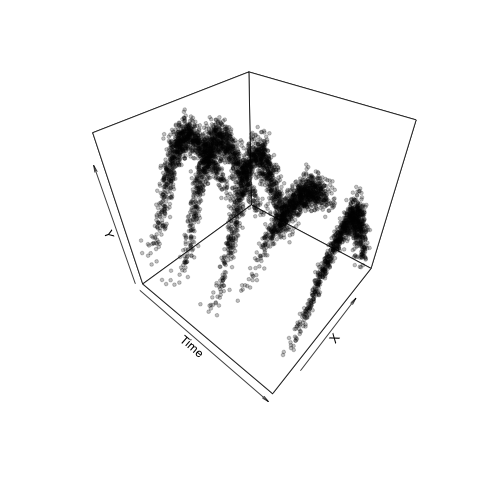
\includegraphics[scale=0.4]{sim_case1_plot2}
  \caption{Longitudinal Simulated Data with $D = 2$. Data from the functions $x_1 = r$ and $x_2 = \alpha\sin(\beta r + \frac{\pi}{2})$ are simulated at 5 time points. Random noise is added both in time and space as $\zeta \mathbf{g}(t) + \iota$, where $\mathbf{g}(t)$ represents a normally distributed spatial translation applied to all points at each time point, and $\iota$ represents normally distributed noise applied to each point individually.}
  \label{fig:sample_data}
\end{figure}

Assume that our goal is estimation of a smooth surface for the brain region of interest at each time point such that the changes of the surface over time are smooth. It is important for the resulting manifolds to be estimated at each time point in order to enable further inference, i.e. modeling trajectories of change in region volumes over time, identifying regions that are most affected in terms of atrophy, etc. The key reasons why the existing principal manifold estimation methods cannot be implemented in this setting are 1) if we implement the data reduction method above then the resulting principal manifold will not be a function of time $t_j$, which is necessary for the resulting segmentations to be useful in practice, 2) if the manifold is estimated separately at each time point, the results may not be smooth over time. In other words, the dimension reduction should be implemented to obtain the 2-dimensional coordinates $(y_1,y_2,t_j)$ while ensuring that the resulting manifold is also a function of $t_j$. In order to address the limitations of the existing approaches for the setting described above, we now propose longitudinal principal manifold estimation (LPME) algorithm to estimate $d$-dimensional representations of $D$-dimensional objects observed over time. 

To give a more general representation of this problem, let $\left\{\bm{x}_i\right\}_{i=1, t=1}^{I_t, T}$ represent the $I = \sum_{t=1}^{T}I_t$ $D$-dimensional observations for each individual, where $I_t$ denotes the number of observations available at each time point, with $T$ total time points. As in the setting described above, at each time point $t$, these observations lie along a $d$-dimensional manifold and are corrupted by $D$-dimensional noise. However, in this updated case, the function determining the manifold may change over time.

\subsection{The Longitudinal Principal Manifold Framework}

Suppose the $d$-dimensional manifold of interest depends on time $t$, which can be represented by a function $F(r,t)$ defined on the ``spacetime" $\mathbb{R}^d\times\mathbb{R}$, where $\mathbb{R}^d$ and $\mathbb{R}$ correspond to ``space" and ``time," respectively. For each fixed time point $t$, the function $f_t(r):=F(r,t)$ of $r$ is the manifold of interest, e.g. the surface of the 3D brain region, at time $t$. 
\begin{definition}
  \label{def:lpme} Given a random $D$-vector $\boldsymbol{X}_t$ observed over time, $\boldsymbol{X}$ denotes the collection of data clouds observed at all time points, such that the manifold $M_F^{d+1}$ is representative of $\boldsymbol{X}$ and for given tuning parameters $\lambda=\{\lambda_t\}_{t\in\mathbb{R}}$ and $\gamma$, let the functional $\mathcal{K}_{\lambda, \gamma, \mathbb{P}}(F)$ be defined as follows. 
\begin{align}\label{eq:newKappa}
  \mathcal{K}_{\lambda, \gamma, \mathbb{P}}(F) &= \int_\mathbb{R} \mathbb{E}\left\|\boldsymbol{X}_t - f_t\left(\pi_{f_t}(\boldsymbol{X}_t)\right)\right\|_{\mathbb{R}^{D}}^2 \, dt + \int_\mathbb{R} \lambda_t \cdot\|\nabla^{\otimes 2}f_t\|_{L^2(\mathbb{R}^{d})}^2 \, dt + \gamma\cdot \int_{\mathbb{R}}\left\|\frac{\partial^2}{\partial t^2}f_t\right\|_{L^2(\mathbb{R}^d)}^2 \, dt \\
  &= \int_{\mathbb{R}}\mathcal{K}_{\lambda_t, \mathbb{P}}(f_t) \, dt + \gamma \cdot \int_{\mathbb{R}}\left\|\frac{\partial^2}{\partial t^2}f_t\right\|_{L^2(\mathbb{R}^d)}^2 \, dt. \nonumber
\end{align}
where $F \in C(\mathbb{R}^{d}\times\mathbb{R} \to \mathbb{R}^{D})$, such that $\lim_{\|r\|_{\mathbb{R}^{d}} \to \infty, t \to \infty}\|F(r,t)\|_{\mathbb{R}^{D}} = \infty$ and the elements of the function $F$ are in $\nabla^{-\otimes 2}L^2(\mathbb{R}^{d}\times\mathbb{R}) = \left\{u \in \mathcal{D}'(\mathbb{R}^{d}): \|\nabla^{\otimes 2} u\|_{\mathbb{R}^{d \times d}} \in L^2(\mathbb{R}^{d}\times\mathbb{R})\right\}$. Then the manifold $M_{F^{*}}^{d+1}$ is the longitudinal principal manifold of $\boldsymbol{X}$ if $F_{\lambda}^{*} = \argmin_{F}\mathcal{K}_{\lambda, \gamma, \mathbb{P}}(F)$.
\end{definition}

By minimizing the functional $\mathcal{K}_{\lambda, \gamma, \mathbb{P}}$ in (\ref{eq:newKappa}), our goal is to minimize the distance between each data point and its projection on the fitted manifold at each time point $t$, penalize the roughness of the fitted manifold at each time point $t$ depending on the value of the tuning parameter $\lambda_t$, and impose smoothness of the function $F$ over time regulated by the tuning parameter $\gamma$. These goals correspond to minimizing the first, second, and third additives of the functional $\mathcal{K}_{\lambda, \gamma, \mathbb{P}}$ in (\ref{eq:newKappa}), respectively. Our proposed framework is based on considering smoothing at a fixed time point and smoothing over time as different problems needing differing solutions. Hence, this approach is different from a thin plate spline or other dimension reduction methods, which would smooth over both the manifold and time jointly or reduce the dimension of space and time together. Using separate smoothing parameters provides additional flexibility in situations where a manifold with a high level of roughness shows minimal changes over time, or vice versa. Generally, our proposed framework can be used in applications where a subset of variables of interest is high-dimensional set with low-dimensional representations of interest, while the resulting low-dimensional representations may be considered to be smooth over the other set of variables. 







\subsection{The LPME Algorithm}

Given the framework proposed in the previous section, estimation of the longitudinal principal manifold entails minimizing the function in (\ref{eq:newKappa}). Our proposed algorithm is based on a multi-stage approach, where we consider smoothing of the data clouds at each time point (spatial smoothing) and then smoothing of the obtained manifolds over time (temporal smoothing). At each individual time point we assume that a manifold has been fit to the data cloud using a spline-based mapping. Hence, in the spatial smoothing phase we assume that we have a collection of spline coefficients that can be used to project from the low-dimensional parameterization to the high-dimensional space. For example, the PME algorithm can be used to obtain this parameterization. In the LPME algorithm, we then use these low-dimensional representations at each time point as the outcomes in a thin plate spline, smoothing over the spatial spline coefficients with respect to time. This yields a multi-stage model that, for a provided time point and set of tuning parameters, obtains a set of spline coefficients that are time-dependent, then returns the high-dimensional output of the spline function associated with the tuning parameter set. Our proposed LPME algorithm consists of four steps: data reduction, initialization, fitting, and tuning. A visualization of these steps is shown in Figure \ref{fig:lpme_steps}. Details of this approach are described below and formally given in Algorithm \ref{alg:lpme}, and an implementation is available as an \texttt{R} package at \texttt{https://github.com/rjzielinski/pme}.

\begin{figure}[ht]
  \centering
  \subfloat[\centering Data]{{\label{fig:lpme_step1} 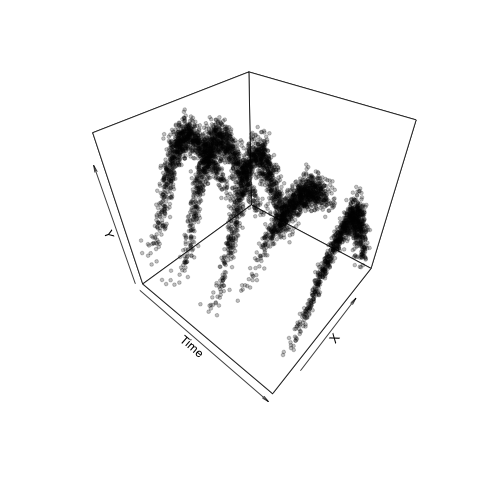
\includegraphics[width=8cm]{sim_case1_plot2}}}%
  \hfill
  \subfloat[\centering Step 1: Sample Size Reduction]{{\label{fig:lpme_step2} 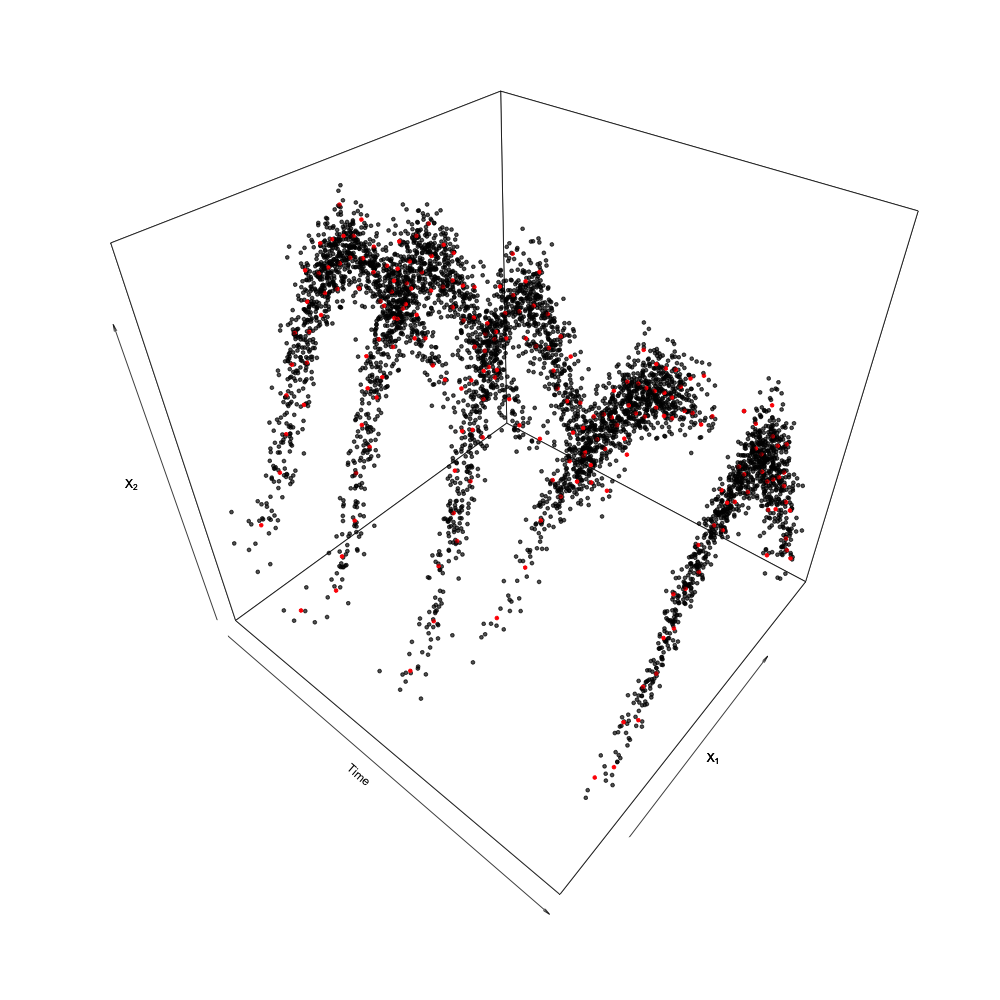
\includegraphics[width=8cm]{lpme_data_reduction}}}
  \vfill
  \subfloat[\centering Step 2: Initialization]{{\label{fig:lpme_step3} 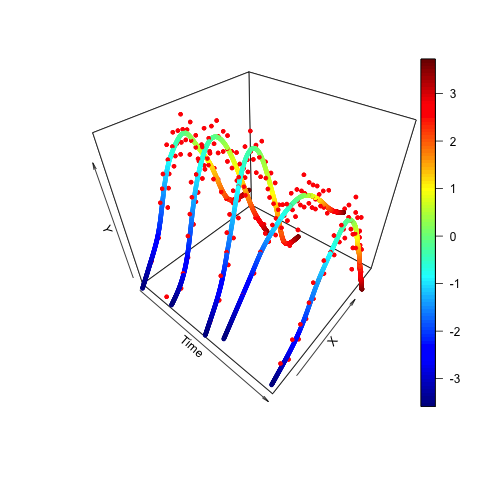
\includegraphics[width=8cm]{lpme_initialization}}}
  \hfill
  \subfloat[\centering Steps 3 and 4: Fitting and Tuning]{{\label{fig:lpme_step4} 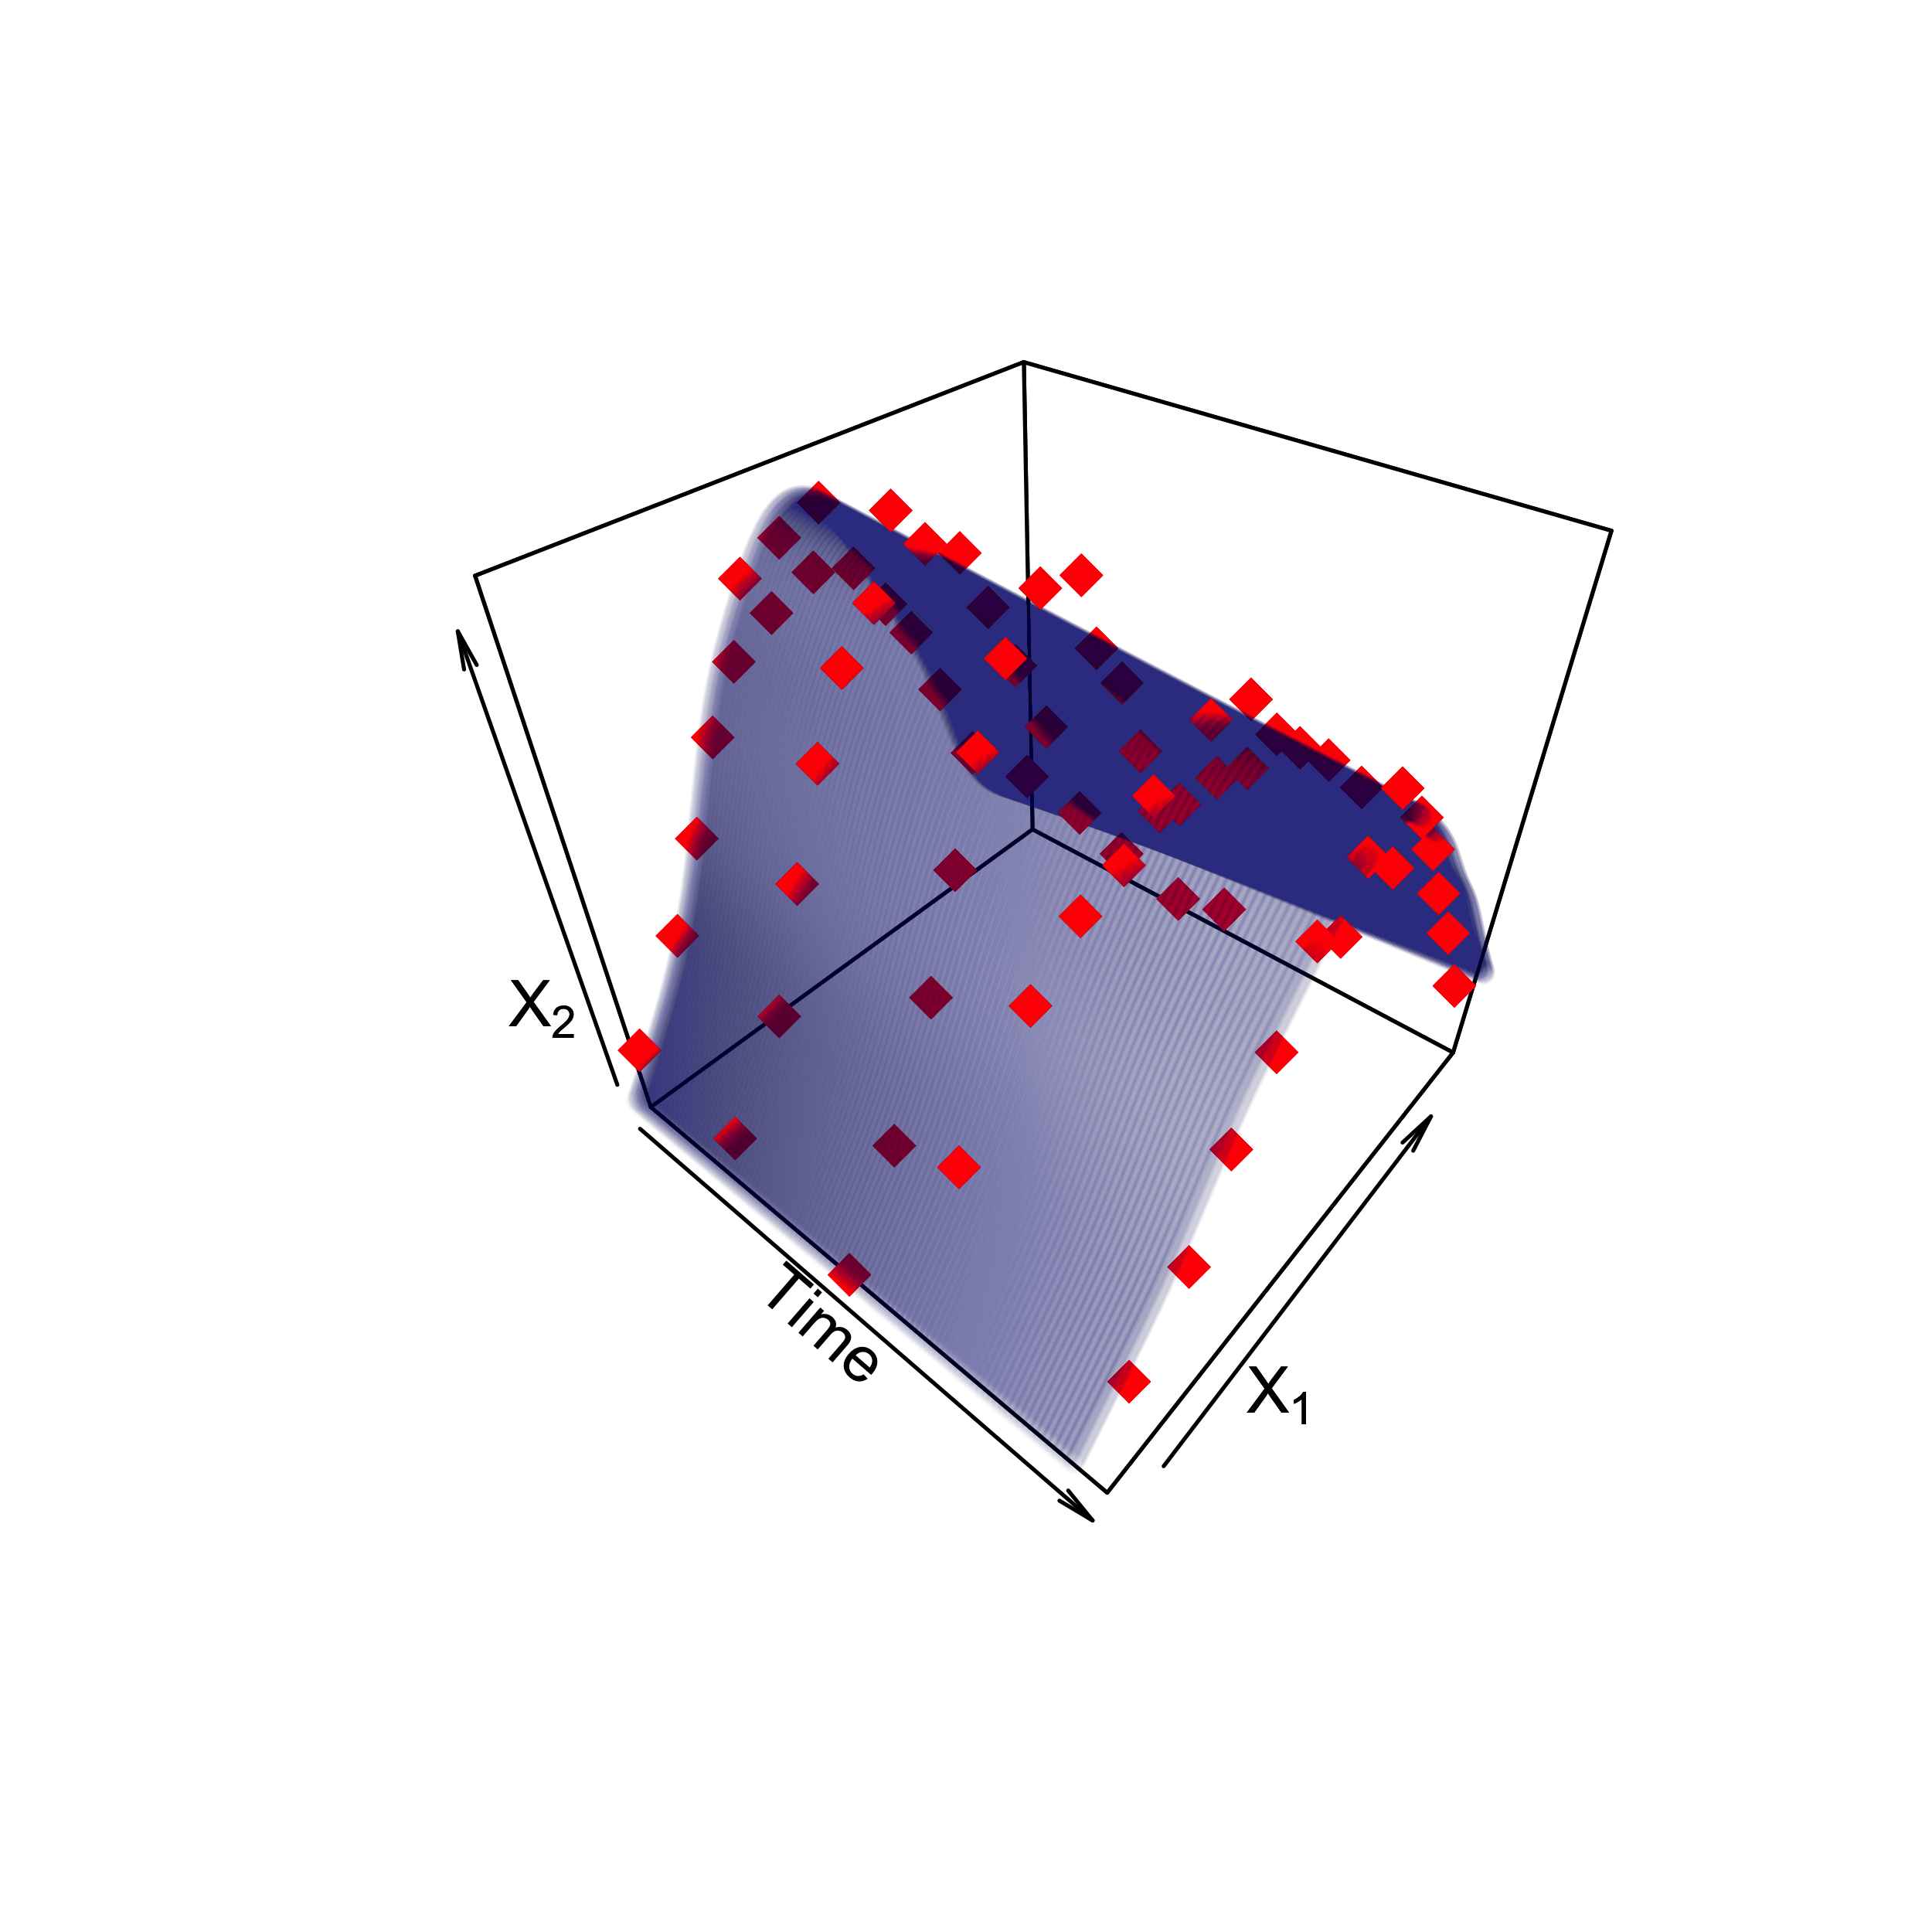
\includegraphics[width=8cm]{lpme_fitting}}}
  \caption{LPME Algorithm Steps. In (a) we show the original data cloud, in (b) we show the sample size reduction step, where the red points indicate the representative data to be used for the next steps of the algorithm, (c) shows the fitted time specific curves, the blue surface in (d) shows the estimated smooth surface. }
  \label{fig:lpme_steps}
\end{figure}


\subsection*{Sample Size Reduction}

In most practical manifold learning tasks data are often quite large, so we begin by implementing an approach for selecting a small number number of points in $D$-dimensional space that represent the structure of the data cloud. This approach is aimed at reducing the sample size of the original data, while maintaining the available information on the curvature of the underlying manifold of interest. Specifically, we consider $D$-dimensional observations $\left\{x_{it}\right\}_{i=1, t=1}^{I_t, T}$ where the sample size $I_t$ is assumed to be large. To reduce the sample size $I_t$, we use the HDMDE method (see \cite{mengPrincipalManifoldEstimation2021}, Section 5.3) to estimate a reduced set of points in the $D$-dimensional space that represent the shape of the data cloud $\left\{x_{it}\right\}_{i=1, t=1}^{I_t, T}$. Briefly, this approach is based on clustering of the original time points to obtain cluster centers, $\left\{\mu_{j, t}\right\}_{j=1, t=1}^{N_t, T}$, represented using red dots in Figure \ref{fig:lpme_step2}, along with their corresponding weights $\{\hat{\theta}_{j, t}\}_{j=1, t=1}^{N_t, T}$ that provide necessary information to characterize the shape of the original data. The number of clusters is estimated for each time point and is allowed to vary among time points to accommodate potential changes in the shape of the underlying structure. By implementing this approach, we reduce the size $\sum_{t=1}^T I_t$ of data $\left\{x_{it}\right\}_{i=1, t=1}^{I_t, T}$ from $I_t$ to $\sum_{t=1}^T N_t$, where each $N_t$ tends to be much smaller than the corresponding $I_t$ (see the simulation study presented in Figure 3(c) of \cite{mengPrincipalManifoldEstimation2021}). The centers estimated in this step are then used to reach an initial low-dimensional parameterization.

\subsection*{Initialization}

The next step in the algorithm for estimation of the longitudinal principal manifold is initialization. Different algorithms use different approaches for this step. For example, the PME algorithm uses Isomap (\cite{tenenbaumGlobalGeometricFramework2000}) to develop an initial parameterization, which the algorithm proceeds to iteratively improve. However, implementation of commonly used approaches for initialization without considering the nuances posed by longitudinal data can be problematic. For instance, using ISOMAP to find parameterizations of similarly shaped structures (i.e. the brain region of interest at each time point) is likely to result in inconsistent parameterization directions across time points (i.e. low values in the parameter space may be associated with low values in the embedding space for one run, while low values in the parameter space may be associated with high values in the embedding space in another). This is demonstrated in Figure \ref{fig:inconsistent_parameterization}, which shows differences in parameterizations depending on the time points of the data cloud presented in Figure \ref{fig:sample_data}. Reaching a successful fit in the LPME algorithm requires consistent parameterizations across time points, so a different approach to generating an initial parameterization is needed. 

\begin{figure}[h]
  \centering
  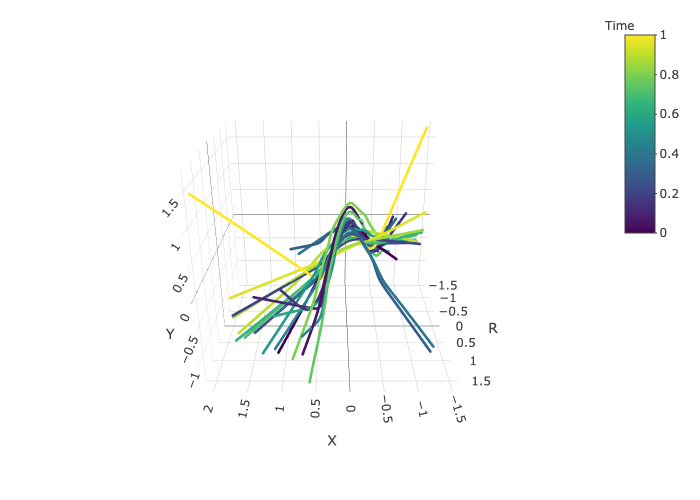
\includegraphics[height=7cm]{inconsistent_parameterization}
  \caption{Simulated data with $D = 2$. The curves shown in this plot represents embedding maps estimated by PME for each time point, with time indicated by the color of the curve. The $X$ and $Y$ axes represent the coordinates of the curve in $D$-dimensional space, while $R$ represents the estimated parameters associated with these coordinates. Randomness in the initialization of the PME algorithm may result in misaligned parameterizations of the estimated embedding maps. For most functions, the $X$ values increase with increasing values for $R$. However, two functions have $X$ values that decrease with increasing $R$. The coefficients for these two functions deviate enough from the other function coefficients that smoothing over the functions with respect to time becomes much more difficult.}
  \label{fig:inconsistent_parameterization}
\end{figure}

To obtain the same parameterization of the manifold over time, instead of using Isomap at each time point separately, we propose using PME to develop a parameterization of the data taken from the first time point, then using the projection index associated with this estimate to find initial parameterizations of the centers for the remaining time points. This approach is based on the assumption that the shape of the structure remains relatively stable over time. In Section \ref{s:simulations}, we show that this process ensures that the initial parameterization remains consistent over time under the assumption of relative stability of the shape of the structure, and we consider some deviations from this assumption and their effect on the results. 

\subsection*{Fitting}

Once the initial parameterization for each cluster center is obtained, the model fitting process begins by using the cluster centers, weights and parameterizations associated with each time point to initialize a PME run. This results in an estimated principal manifold $\widehat{f_t}$ for each time point $t$ and an optimal tuning parameter $\lambda_t^*$ corresponding to the first two terms of the $\mathcal{K}_{\lambda, \gamma, \mathbb{P}}(F)$ defined in \eqref{eq:newKappa} and presented using multicolored lines in Figure \ref{fig:lpme_step3}. The fit of each $\hat{f}_t$ is measured using $\tau_t$, an estimate of the mean squared distance between the observed data points and their projections to the manifold defined by $\hat{f}_t$. At this stage, the time-specific manifolds require further smoothing considering the curvature in the time dimension corresponding to the third term of $\mathcal{K}_{\lambda, \gamma, \mathbb{P}}(F)$. The principal manifold $\widehat{f_t}$ at time $t$ is characterized by spline coefficients. Hence, we estimate a spline function mapping from the time dimension to the coefficient space that smooths over the coefficients for these principal manifolds, given a tuning parameter $\gamma$.

At each time point, the estimated principal manifold has a spline form. As detailed by \cite{greenSilverman1994}, smoothing splines can be considered to have knots at the points used to fit them. This means that, in order for the coefficients of the manifolds estimated at each time point to be comparable, the parameter values used as inputs when the functions were fitted must be identical. Hence, to obtain coefficients that can be compared across time points, a grid of values $\left\{\boldsymbol{r}_i\right\}_{i=1}^{N}$ ($\subset\mathbb{R}^d$) ranging from the minimum to the maximum of the parameters in each of the $d$ dimensions is input into the estimated embedding functions $\widehat{f_t}$ for each time point, with $N$ specified based on the maximum number of clusters identified in the data reduction step at any time point. This yields a set of outcomes, $\left\{Y_{i,t}\right\}_{i=1, t = 1}^{N, T}$, corresponding to same parameter values at each time point, i.e., $Y_{i,t}=\widehat{f_t}(\boldsymbol{r}_i)$ for all $i$ and $t$. Following the discussion in Chapter 7 of \cite{greenSilverman1994}, for each time point $t$, comparable spline coefficients $\boldsymbol{s}_t^*$ and $\boldsymbol{\alpha}_t^*$ can then be calculated by minimizing the following function.
\begin{equation}\label{eq:splineL}
    \mathcal{L}(f_t) = (\boldsymbol{Y}_t - \boldsymbol{E}\boldsymbol{s}_t - \boldsymbol{R}^\T\boldsymbol{\alpha}_t)^\T(\boldsymbol{Y}_t - \boldsymbol{E}\boldsymbol{s}_t - \boldsymbol{R}^\T\boldsymbol{\alpha}_t) + \gamma\boldsymbol{s}_t^\T \boldsymbol{E}\boldsymbol{s}_t
\end{equation}    
where $\boldsymbol{Y}_t$ is the $N \times D$ matrix consisting of elements $\left\{Y_{i,t}\right\}_{i=1}^{N}$ at each time point $t$, the matrix $\boldsymbol{E}=(E_{ij})_{1\le i,j\le N}$ is defined by $E_{ij} = \eta_{d}(\|\boldsymbol{r}_i - \boldsymbol{r}_j\|)$, where $\eta_{d}(r) = r^{4 - d}\log r$ if $d$ is even, and $\eta_d(r) = r^{4-d}$ if $d$ is odd, the functions $\phi_1,\ldots,\phi_{d+1}$ form a basis of the linear space of polynomials on $\mathbb{R}^d$ with degrees $\le1$; and the matrix $\boldsymbol{R}=(R_{ij})_{1\le i\le d+1,1\le j\le N}$ is defined by $R_{ij} = \phi_i(\boldsymbol{r}_j)$.

By computing the derivative of $\mathcal{L}(f_t)$ in (\ref{eq:splineL}), we conduct the minimization of $\mathcal{L}(f_t)$ by solving the following system of equations. 
\begin{equation}
  \left(
    \begin{array}{cc}
      \boldsymbol{E} + \lambda_t^* \boldsymbol{I} & \boldsymbol{R}^\T \\
      \boldsymbol{R} & \boldsymbol{0}
    \end{array}
  \right)\left(
    \begin{array}{c}
      \boldsymbol{s}_t \\
      \boldsymbol{\alpha}_t
    \end{array}
  \right) = \left(
    \begin{array}{c}
      \boldsymbol{Y}_t \\
      \boldsymbol{0}
    \end{array}
  \right). \label{eq:13}
\end{equation}
The solution to Eq.~\eqref{eq:13} , denoted by $\boldsymbol{\alpha}^*_t=(\alpha^*_{1,t},\ldots,\alpha^*_{d+1,t})^\T$ and $\boldsymbol{s}^*_t=(s^*_{1,t},\ldots,s^*_{N,t})^\T$, yields function
\begin{equation}\nonumber
  f_t^*(r) = \sum_{j=1}^{N}s_{j,t}^* \cdot  \eta_{d}\left(\|r - r_j^*\|\right) + \sum_{k=1}^{d + 1}\alpha_{k,t}^* \cdot \phi_k(r). 
\end{equation}

We denote the manifold coefficients at each time point $t$ as $\boldsymbol{\omega}_t = (\boldsymbol{s}_t^{*\T}, \boldsymbol{\alpha}_t^{*\T})^\T$. To limit the ability of a poorly-fitting PME estimate to greatly influence the results of the LPME model, we fit a weighted spline model to smooth over the manifold coefficients, where the weights for each time point $t$ are equal to 
$$w_t = \frac{1}{\tau_t\sum_{i=1}^{T}\frac{1}{\tau_i}}.$$ 

With a given tuning parameter value $\gamma$, we then fit a weighted cubic spline function using $\left\{t_i\right\}_{i=1}^T$ as predictors and $\left\{\mathbf{\omega}_t\right\}_t$ as the response values, with weights $\left\{w_t\right\}_t$ resulting in a function taking the form
\begin{equation}\nonumber
  g_{\gamma}(t) = \sum_{i=1}^{T}\delta_i \,\|t - t_i\|^{3} + \sum_{j=1}^{2}\nu_j\,\phi(t)_j,
\end{equation}
where by defining the $T \times T$ matrix $\boldsymbol{A}$ as defined  $\boldsymbol{A}_{ij} = \|t_i - t_j\|^{3}$ with $i,j = 1,\ldots, T$, the matrix $\boldsymbol{T}$ as defined $\boldsymbol{T}_{ij} = \phi_i(t_j)$, and $\boldsymbol{W} = \operatorname{diag}(w_1, \dots, w_T)$,  $\boldsymbol{\delta}=(\delta_1,\ldots,\delta_T)^\T$ and $\boldsymbol{\nu}=(\nu_1,\nu_2)^\T$ are the solutions to 
\begin{equation}
  \left(
  \begin{array}{ccc}
    2\boldsymbol{A}\boldsymbol{W}\boldsymbol{A} + 2\gamma\boldsymbol{A} & 2\boldsymbol{A}\boldsymbol{W}\boldsymbol{T} & \boldsymbol{T} \\
    2\boldsymbol{T}^{T}\boldsymbol{W}\boldsymbol{A} & 2\boldsymbol{T}^{T}\boldsymbol{W}\boldsymbol{T} & \boldsymbol{0} \\
    \boldsymbol{T}^{T} & \boldsymbol{0} & \boldsymbol{0}
  \end{array}
  \right)\left(
  \begin{array}{c}
    \boldsymbol{\delta} \\
    \boldsymbol{\nu} \\
    \boldsymbol{m}
  \end{array}
  \right) = \left(
  \begin{array}{c}
    2\boldsymbol{A}\boldsymbol{W}\boldsymbol{\Omega} \\
    2\boldsymbol{T}^{T}\boldsymbol{W}\boldsymbol{\Omega} \\
    \boldsymbol{0}
  \end{array}
  \right), \label{eq:16}
\end{equation}
where $\boldsymbol{\Omega}=(\boldsymbol{\omega}_1,\ldots, \boldsymbol{\omega}_T)^\T$.

With $\gamma$ given, we denote the manifold coefficients at time $t$ estimated by function $g(\cdot)$ as $\boldsymbol{\Omega}_{\gamma}(t) = \left(\boldsymbol{s}_{\gamma}(t)^\T, \boldsymbol{\alpha}_{\gamma}(t)^\T\right)^\T$. Hence, given $\gamma$, the estimated embedding function given time $t$ and $d$-dimensional parameterization $\boldsymbol{r}$ may be written as
\begin{equation}
  F_{\gamma}(t, \boldsymbol{r}) = \sum_{j=1}^{N}\boldsymbol{s}_{\gamma}(t)_j \eta_{d}\left(\|\boldsymbol{r} - \boldsymbol{r}_j^*\|\right) + \sum_{k=1}^{d+1}\boldsymbol{\alpha}_{\gamma}(t)_k \phi_k(\boldsymbol{r}). \label{eq:17}
\end{equation}


\subsection*{Tuning}

Once $F_{\gamma}(t, \boldsymbol{r})$ have been estimated for all provided tuning values, the optimal tuning parameter $\gamma^*$ is identified using leave-one-out cross validation. In this process, the coefficient smoothing function is computed while excluding all data and coefficients with time $t$ from consideration, for $t = 1, \dots, T$. We denote this function by $g_{\gamma}^{(t)}$. We can then assess the performance of the LPME model using tuning value $\gamma$ by averaging over estimates of MSD calculated using the original observations associated with the left-out time $t$ as follows.
\begin{equation}
  MSD(\gamma) = \frac{1}{T} \sum_{t=1}^{T}\frac{1}{I_t}\sum_{i=1}^{I_t}\|x_{i, t} - f_{\gamma}^{(t)}(t, \pi_{f_{\gamma}^{(t)}}(x_{i, t}))\|^2. \label{eq:18}
\end{equation}
The optimal tuning value $\gamma^*$ is then found to be the value of $\gamma$ that minimizes $MSD(\gamma)$. Note that alternative cross validation methods, such as $k$-fold cross validation, could easily be used in place of leave-one-out cross validation to better meet computational demands. 

%\meng{Do some simulation studies and compare the leave-one-out CV and k-fold CV.}

\RestyleAlgo{ruled}
\LinesNumbered

\SetKwComment{Comment}{/* }{ */}

\RestyleAlgo{ruled}
\LinesNumbered



\begin{algorithm}
\caption{Longitudinal Principal Manifold Estimation}\label{alg:lpme}
  \KwData{Data points $\left\{X_{i, t}\right\}_{i=1, t=1}^{I_t, T}$, positive integer $d$, positive integer $N_0 < \min{I_t} - 1$, $\alpha$, $\epsilon$, $\epsilon^* \in (0, 1)$, candidate tuning parameters $\left\{\lambda_k\right\}_{k=1}^K$, $\left\{\gamma_l\right\}_{l=1}^L$, $itr \geq 1$, which is the maximum number of iterations allowed.}
\KwResult{Analytic formula of $\hat{f}^*: \mathbb{R}^{d + 1} \to \mathbb{R}^{D + 1}$, optimal tuning parameter $\gamma^*$.}
\For{$t = 1, 2, \dots, T$} {
  Apply HDMDE algorithm with input $\left(\left\{X_{i, t}\right\}_{i = 1}^{I_t}, N_0, \epsilon, \alpha\right)$ and obtain $N_t$, $\left\{\mu_{j, t}\right\}_{j = 1}^{N_t}$, and $\left\{\theta_{j, t}\right\}_{j = 1}^{N_t}$\;
}

  Apply PME to parameterize $\left\{\mu_{j, 1}\right\}_{j = 1}^{N_1}$ by the $d$-dimensional parameters $\left\{r_{j, t}\right\}_{j = 1}^{N_1}$ and use $\pi_{f_1(0)}$ to parameterize $\left\{\mu_{j, t}\right\}_{j=1, t = 1}^{N_t, T}$ by $\left\{r_{j, t}\right\}_{j=1, t=2}^{N_t, T}$. Formally set $\pi_{f_1(0)}(\mu_{j, 1}) \gets r_{j, 1}$ for $j = 1, 2, \dots, N_1$, and $\pi_{f_{t}(0)}(\mu_{j, t}) \gets \pi_{f_1(0)}(\mu_{j, t})$ for $j = 1, 2, \dots, N_t$, $t = 2, \dots, T$\;

\For{t = 1, 2, \dots, T} {
  Apply modified PME algorithm with $\pi_{f_t(0)}(\mu_{j, N_t, t}) \gets \left\{r_{j, t}\right\}_{j = 1}^{N_t}$ and obtain $f_t$, $\lambda_t^*$, and $\tau_t$\;
  $\left\{r_{j, t}\right\} \gets \pi_{f_t}(\mu_{j, t})$ for $j = 1, \dots, N_t$ and $Y_{j, t} \gets f_t(r_{j, t})$ for $j = 1, \dots, N_t$\;
}

  Let $N = \max(N_t)$, $\left\{r_i^*\right\}_{i=1}^{N}$ be a grid spanning the range of estimated values of $\left\{r_{i, j}\right\}_{i=1, t=1}^{N_t, T}$\; 

\For{t = 1, 2, \dots, T} {
  Set $Y_{i, t} = f_t(r_{i}^*)$ for $i = 1, \dots, N$\;
  Compute $f_t^*(r)$ by solving \eqref{eq:13}\;
  Set $w_t = \frac{1}{\tau_t \sum_{i=1}^{T}\frac{1}{\tau_i}}$\;
}

  Define $\boldsymbol{\omega}$ by setting $\boldsymbol{\omega}_t = \left[\boldsymbol{s}_t, \boldsymbol{\alpha}_t\right]$\;
  \For{l = 1, 2, \dots, L} {
    Compute $g_{\gamma_l}(t)$ by solving \eqref{eq:16}\;
    \For{t = 1, 2, \dots, T} {
      Compute $g_{\gamma_l}^{(t)}$ by solving \eqref{eq:16}\;
    }
    Estimate $MSD(\gamma_l)$ using \eqref{eq:18}\;
  }
  $\gamma^* = \arg\min_{\gamma}MSD(\gamma)$\;
  $f^*(t, \boldsymbol{r}) = f_{\gamma^*}(t, \boldsymbol{r})$, where the form of $f^*(t, \boldsymbol{r})$ is given in \eqref{eq:17}
\end{algorithm}


\subsection{Self-intersecting Manifold Estimation}\label{ss:selfInt}

Notably, in many applications where manifold learning is implemented, the high-dimensional shapes of interest are self-intersecting manifolds. Methods based on the principal curve framework, including the principal manifold approach used here, are typically unable to fit such manifolds due to the self-consistency condition introduced in \cite{hastiePrincipalCurves1989}. To avoid this issue, we propose a data augmentation approach with polar or spherical coordinates, depending on the value of $D$. As a simple example, the unit circle can be considered a self-intersecting manifold with $d = 1$ when viewed in two dimensions. However, by adding a third dimension equal to the angle of each observation from the origin, the manifold can be considered as having $d = 1$ and $D = 3$, while avoiding any self-intersections. This enables the PME algorithm, and thus the LPME algorithm, to be fit under these circumstances. This process is illustrated graphically in Figure \ref{fig:unit_circle_augmentation}. 

\begin{figure}[ht]
  \centering
  \subfloat[\centering Unaugmented Unit Circle]{{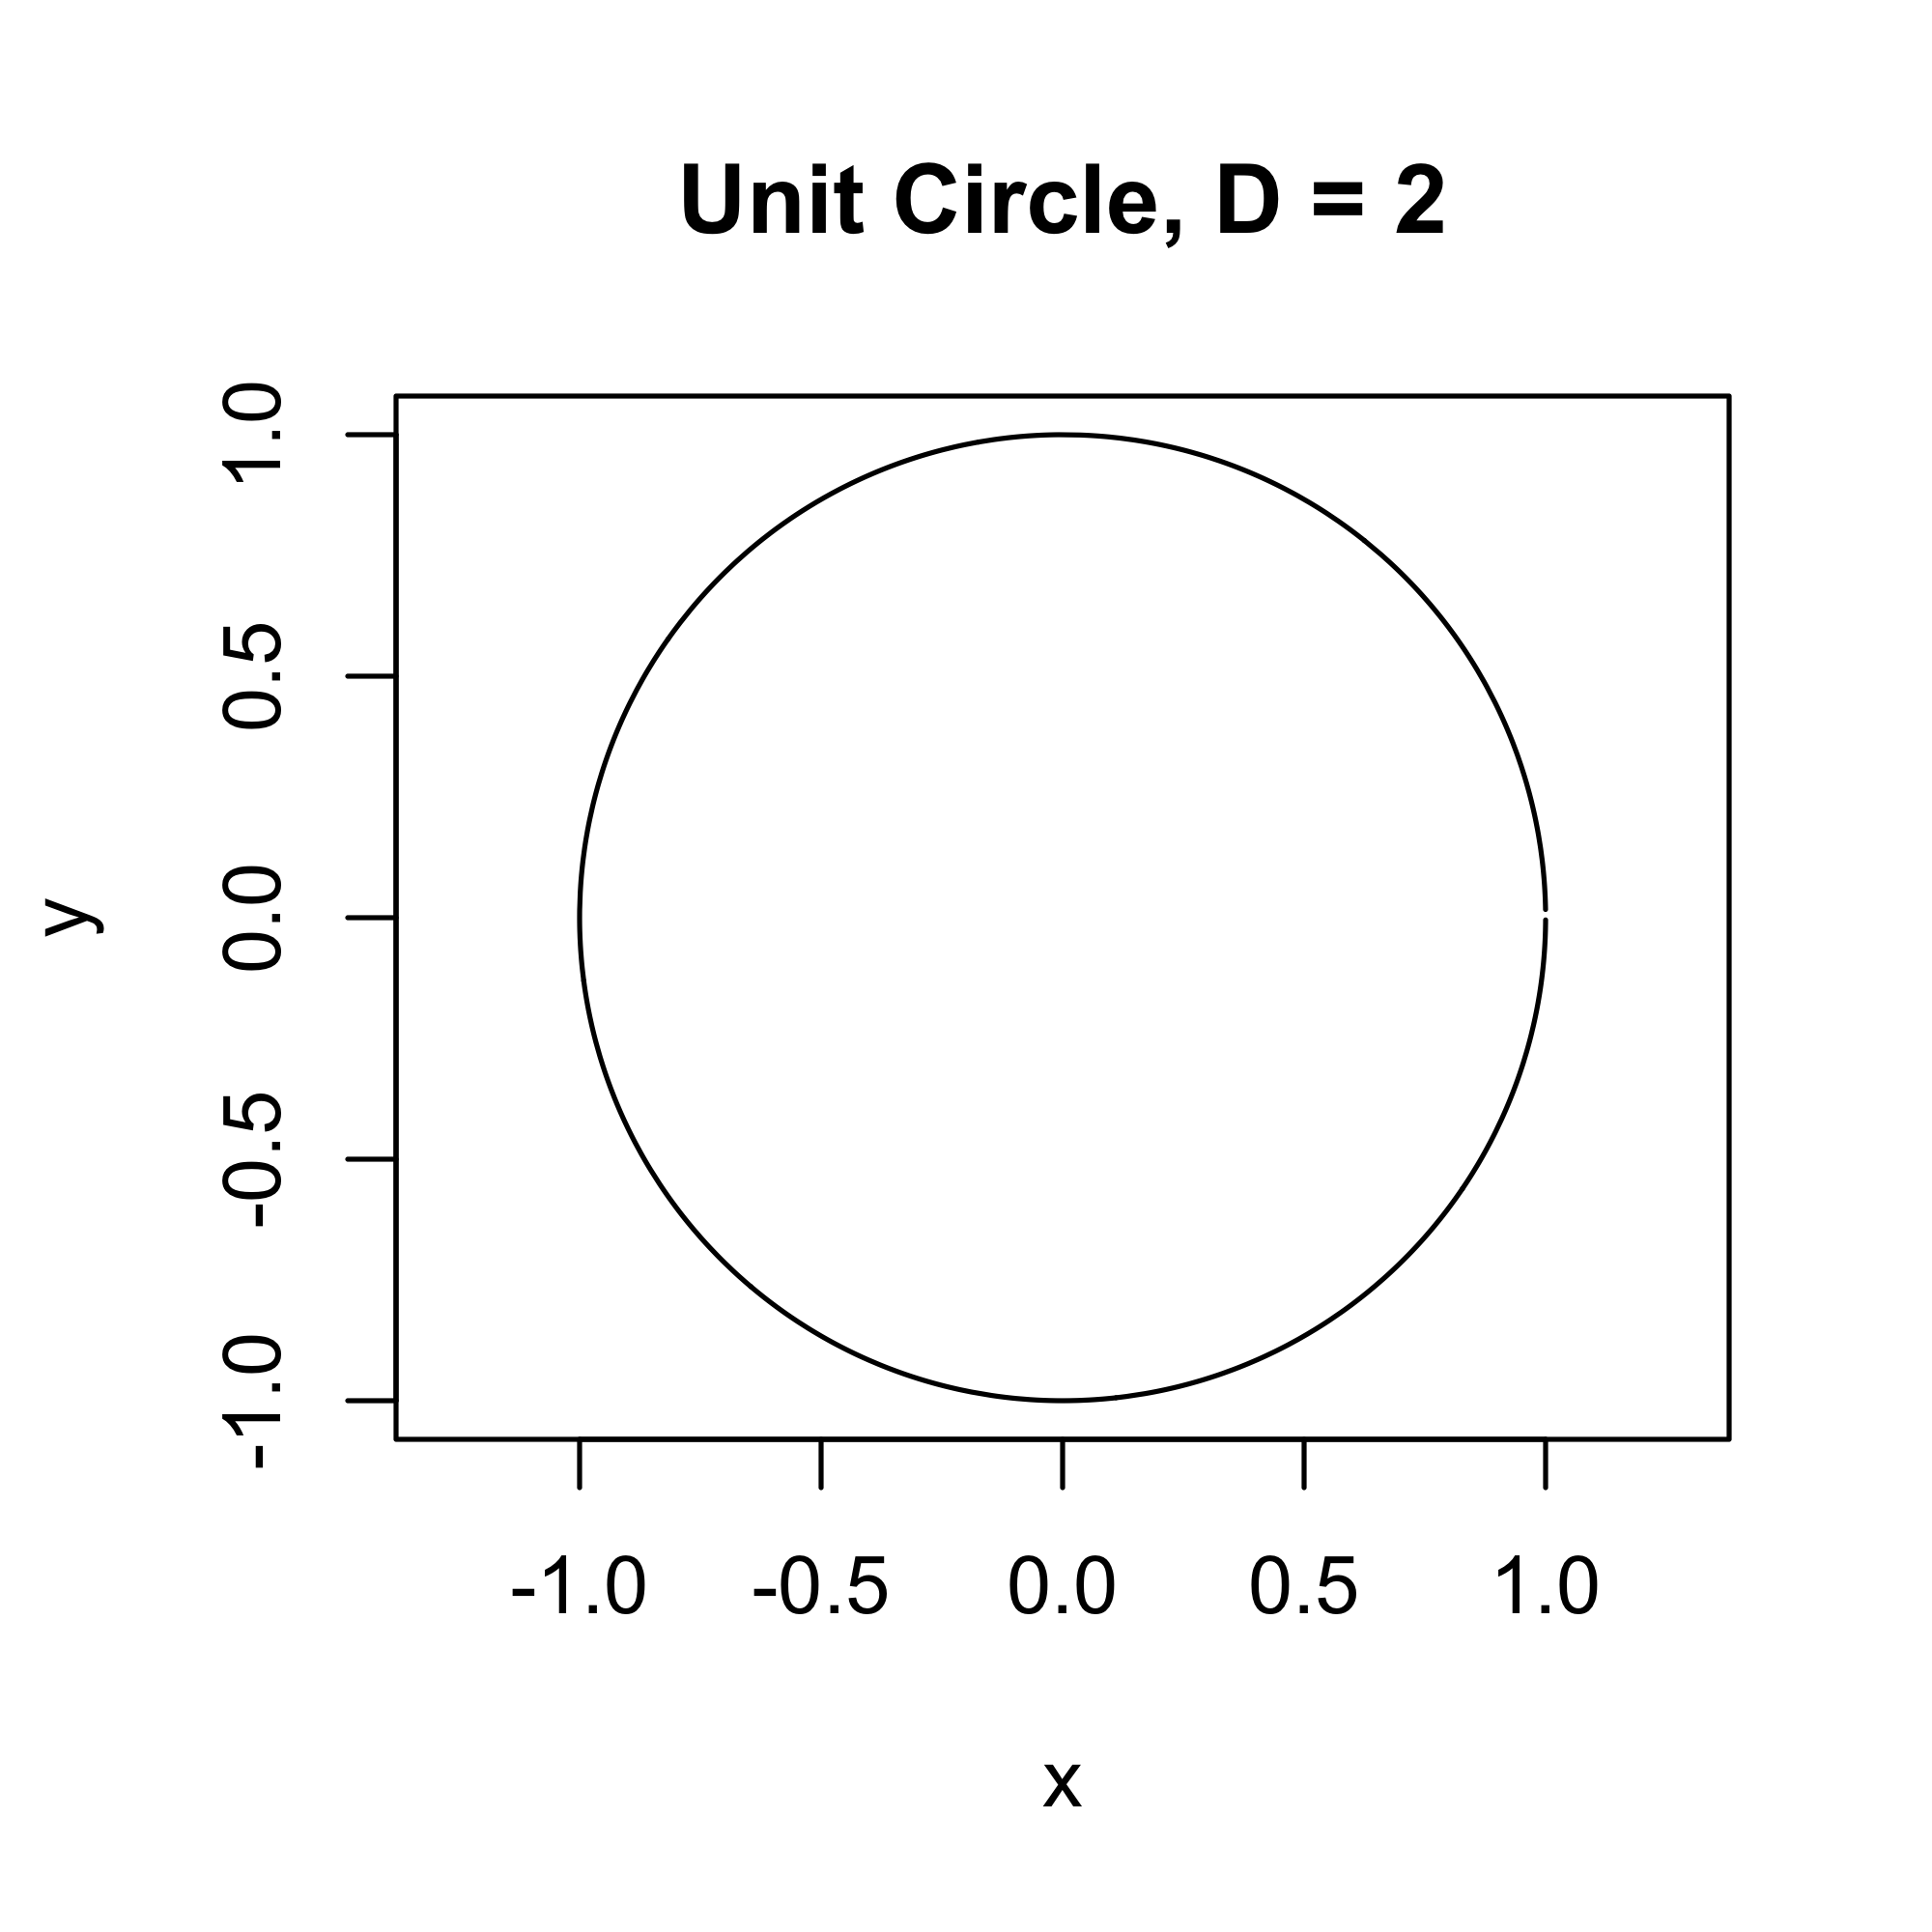
\includegraphics[width=9cm]{unit_circle_D2}}}%
  \hfill
  \subfloat[\centering Augmented Unit Circle]{{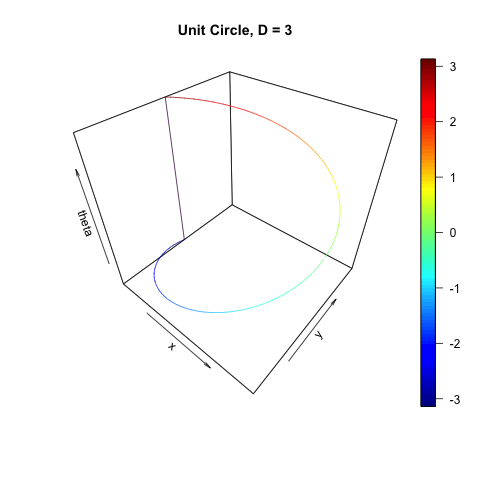
\includegraphics[width=9cm]{unit_circle_D3}}}
  \caption{Illustration of our proposed data augmentation approach using the Unit Circle. The left panel (a) shows the depiction of the circle with $d=1$ and $D=2$, while the right panel (b) shows how our proposed use of considering this same manifold in $D=3$ by using the spherical coordinates results in a manifold that is not self-intersecting.}
  \label{fig:unit_circle_augmentation}
\end{figure}

This approach to data augmentation offers an alternative to the method used in \cite{mengPrincipalManifoldEstimation2021} to fit the PME algorithm to self-intersecting manifolds, where the full dataset was manually partitioned to avoid intersections within each partition. Reaching a combined estimate after fitting PME to each partition individually requires ``gluing'' the estimated manifolds on each partition together, which may introduce error to the combined manifold estimate. This source of error is avoided using our proposed data augmentation approach. Additionally, scaling the added dimensions by a constant value enables the modification of the level of curvature present in the manifold. This may encourage improved performance when estimating manifolds that have too much curvature for PME to reach an appropriate fit under normal circumstances. However, an in depth comparison of these approaches is beyond the scope of this article and is left for future work.





\section{Simulations}\label{s:simulations}

To assess the performance of the LPME algorithm, we compare its performance with that of two alternative approaches on simulated datasets. We consider settings in which $d = 1$ and $D = 2$, $d = 1$ and $D = 3$, and $d = 2$ and $D = 3$, with several manifolds being used to generate datasets in each setting. For each manifold, we consider differing values for the time duration, interval between observations, noise levels within and between time points, and the type and magnitude of structural changes in the underlying manifold over time. The embedding functions used to define each manifold are given in Table \ref{table:simulation_embeddings}. In these functions, the value of $\zeta$ and the functional form of $g(\cdot)$ are varied between trials and represent structural changes in the underlying manifold over time. The function $g(\cdot)$ may show change with respect to time that is constant, linear, quadratic, or sinusoidal, with $\zeta$ serving as a scalar multiplier. The values of $\iota$ represent within-image noise in the high-dimensional space, and are randomly sampled from a normal distribution with mean zero and variance that is varied between trials. Meanwhile, $\alpha$ and $\beta$ are vectors of length $d$ that are drawn from a normal distribution with mean equal to 1 and variance that is varied between trials. These values describe random fluctuations in the manifold between time points, reflecting noise introduced by different imaging sessions.

\begin{table}[ht]
\small
  \centering
  \begin{tabular}{|c c c c c|}
    \hline
    Case & $d$ & $D$ & $f_t(\mathbf{r})$ & Domain \\
    \hline
    1 & 1 & 2 & $\left(r, \ \alpha \text{sin} \ (\beta r + \frac{\pi}{2})\right) + \zeta\mathbf{g}(t) + \iota$ & $-3 \leq r \leq 3$ \\
    2 & 1 & 2 & $\left(r, \ \alpha\text{sin} \ (\beta r)\right) + \zeta\mathbf{g}(t) + \iota$ & $-3\pi \leq r \leq 3\pi$ \\
    3 & 1 & 2 & $\left(\alpha_1 \text{cos} \ (\beta_1 r), \ \alpha_2\text{cos} \ (\beta_2 r)\right) + \zeta\mathbf{g}(t) + \iota$ & $-\frac{4\pi}{5} \leq r \leq \frac{\pi}{2}$ \\
    4 & 1 & 3 & $\left(r, (\alpha_1r + \beta_1)^2, \ (\alpha_2r + \beta_2)^3\right) + \zeta\mathbf{g}(t) + \iota$ & $-1 \leq r \leq 1$ \\
    5 & 1 & 3 & $\left(r, \ \alpha_1\text{cos} \ (\beta_1 r), \ \alpha_2\text{sin} \ (\beta_2 r) \right) + \zeta\mathbf{g}(t) + \iota$ & $0 \leq r \leq 3\pi$ \\
    6 & 2 & 3 & $\left(\beta_1r_1, \ \beta_2r_2, \ \alpha_1(\alpha_2\|\beta\mathbf{r}\|^2)\right) + \zeta\mathbf{g}(t) + \iota$ & $-1 \leq r_1, r_2 \leq 1$\\
    7 & 2 & 3 & $\left(\alpha_1\beta_1r_1\text{cos} \ (\alpha_1r_1), \ \alpha_2\beta_2r_1\text{sin} \ (\alpha_2r_1), \ r_2\right) + \zeta\mathbf{g}(t) + \iota$ & $0 \leq r_1 \leq 3\pi$; \ $-1 \leq r_2 \leq 1$\\
    8 & 2 & 3 & $\left(\alpha_1\text{sin}(\beta_1r_1)\text{cos}(\beta_2r_2), \ \alpha_1\text{sin}(\beta_1r_1)\text{sin}(\beta_2r_2), \ \alpha_1\text{cos}(\beta_1r_1)\right) + \zeta\mathbf{g}(t) + \iota$ & $0 \leq r_1 \leq \pi$; \ $0 \leq r_2 \leq 2\pi$\\
    \hline
  \end{tabular}
  \caption{Embedding functions used for simulation trials.}
  \label{table:simulation_embeddings}
\end{table}

In the situations where $d = 1$, LPME is compared to the PME method naively run at each time point without smoothing over time, as well as the principal curve algorithm described in \cite{hastiePrincipalCurves1989}, also run independently at each time point. The principal curve algorithm is implemented using the \texttt{principal\_curve()} function in the \texttt{princurve} package, developed using \texttt{R} (\cite{rSoftware2023}). In this function, each of the three smoothing options, \texttt{smooth\_spline}, \texttt{lowess}, and \texttt{periodic\_lowess}, are tested, with the option resulting in the lowest error from the true values being chosen. Following \cite{mengPrincipalManifoldEstimation2021}, the inputs for the PME algorithm are set to $N_0 = 20 \times D$, $\alpha = 0.05$, and $\epsilon = 0.001$, with $\lambda_g = \exp(g)$ for $g = -15, \dots, 5$. In cases where $d = 2$, LPME is again compared to the naive PME approach described above, and the principal surface estimation algorithm developed by \cite{yueParameterizationWhiteMatter2016}.

A factorial design is used to run the simulation studies, with the factor levels set as follows: 1) $\alpha, \beta, \zeta \in \left\{0, 0.05, 0.1, 0.25, 0.5, 1.0\right\}$; 2) study duration: $\left\{1, 2, 5\right\}$; 3) interval between images: $\left\{0.1, 0.25, 0.5\right\}$; 4) longitudinal change model: Constant, Linear, Quadratic, Sinusoidal. The sample size for each time point is set to 1,000 observations, so each embedding map is simulated a total of 7,776 times. All code required to reproduce the simulation results and the associated figures is provided at \href{https://github.com/rjzielinski/lpme-project}{\texttt{https://github.com/rjzielinski/lpme-project}}.

Visualizations of the results from some of the simulation cases, truncated for concision, are shown in Figures \ref{fig:sim_case1} and \ref{fig:sim_case6}. Informally, the performance of each estimation method can be observed by considering the proximity of each method's estimated manifold to the true manifold (shown in red) over time. Thus, in Figure \ref{fig:sim_case1}, we see that the LPME-estimated manifold bears the closest resemblance to the true manifold underlying the data, while the manifolds estimated by PME and the principal curve method show greater responses to temporary random fluctuations in the data at each time point.

\begin{table}[h]
  \centering
  \begin{tabular}{|c c c c c|}
    \hline
    Case & Data & LPME & PME & PC/PS \\
    \hline
    1 & 0.223 (0.256) & {\bf 0.125 (0.161)} & 0.268 (0.850) & 0.189 (0.245) \\
    2 & 0.514 (0.408) & {\bf 0.384 (0.648)} & 0.843 (1.93) & 0.600 (0.296) \\
    3 & 0.446 (0.445) & {\bf 0.401 (0.446)} & 0.507 (0.594) & 0.412 (0.423) \\
    4 & 30.7 (88.1) & {\bf 27.7 (260)} & 30.7 (88.2) & 30.6 (88.1) \\
    5 & 0.980 (0.771) & {\bf 0.791 (0.845)} & 1.04 (1.07) & 0.934 (0.713) \\
    6 & 1.43 (6.04) & 1.21 (5.66) & 1.47 (6.06) & {\bf 1.01 (2.11)} \\
    7 & 0.580 (0.839) & 4.07 (3.30) & 7.37 (1.14) & {\bf 1.95 (0.800)} \\
    8 & 0.226 (0.275) & {\bf 0.136 (0.169)} & 0.242 (0.311) & 0.274 (0.243) \\
    \hline
  \end{tabular}
  \caption{MSD comparison to true values, Mean (SD). For each case, the lowest algorithm-specific mean (SD) are highlighted in bold. }
  \label{table:simulation_results_mean}
\end{table}


\begin{table}[h]
  \centering
  \begin{tabular}{|c c c c c|}
    \hline
    Case & Data & LPME & PME & PC/PS \\
    \hline
    1 & 0.146 (0.233) & {\bf 0.074 (0.122)} & 0.131 (0.258) & 0.118 (0.206) \\
    2 & 0.467 (0.665) & {\bf 0.248 (0.516)} & 0.516 (0.750) & 0.564 (0.419) \\
    3 & 0.291 (0.601) & {\bf 0.239 (0.564)} & 0.317 (0.640) & 0.264 (0.584) \\
    4 & 4.26 (21.2) & {\bf 3.29 (13.0)} & 4.23 (21.1) & 4.22 (21.2) \\
    5 & 0.895 (1.33) & {\bf 0.584 (1.08)} & 0.894 (1.36) & 0.821 (1.22) \\
    6 & 0.284 (1.06) & {\bf 0.273 (0.891)} & 0.316 (1.04) & 0.557 (0.387) \\
    7 & 0.145 (0.552) & 2.96 (4.65) & 6.92 (1.17) & {\bf 1.58 (0.514)} \\
    8 & 0.110 (0.325) & {\bf 0.074 (0.208)} & 0.115 (0.331) & 0.172 (0.234) \\
    \hline
  \end{tabular}
  \caption{MSD comparison to true values, Median (IQR). The lowest algorithm-specific median (IQR) are highlighted in bold.}
  \label{table:simulation_results_median}
\end{table}

\begin{figure}[h]
  \centering
  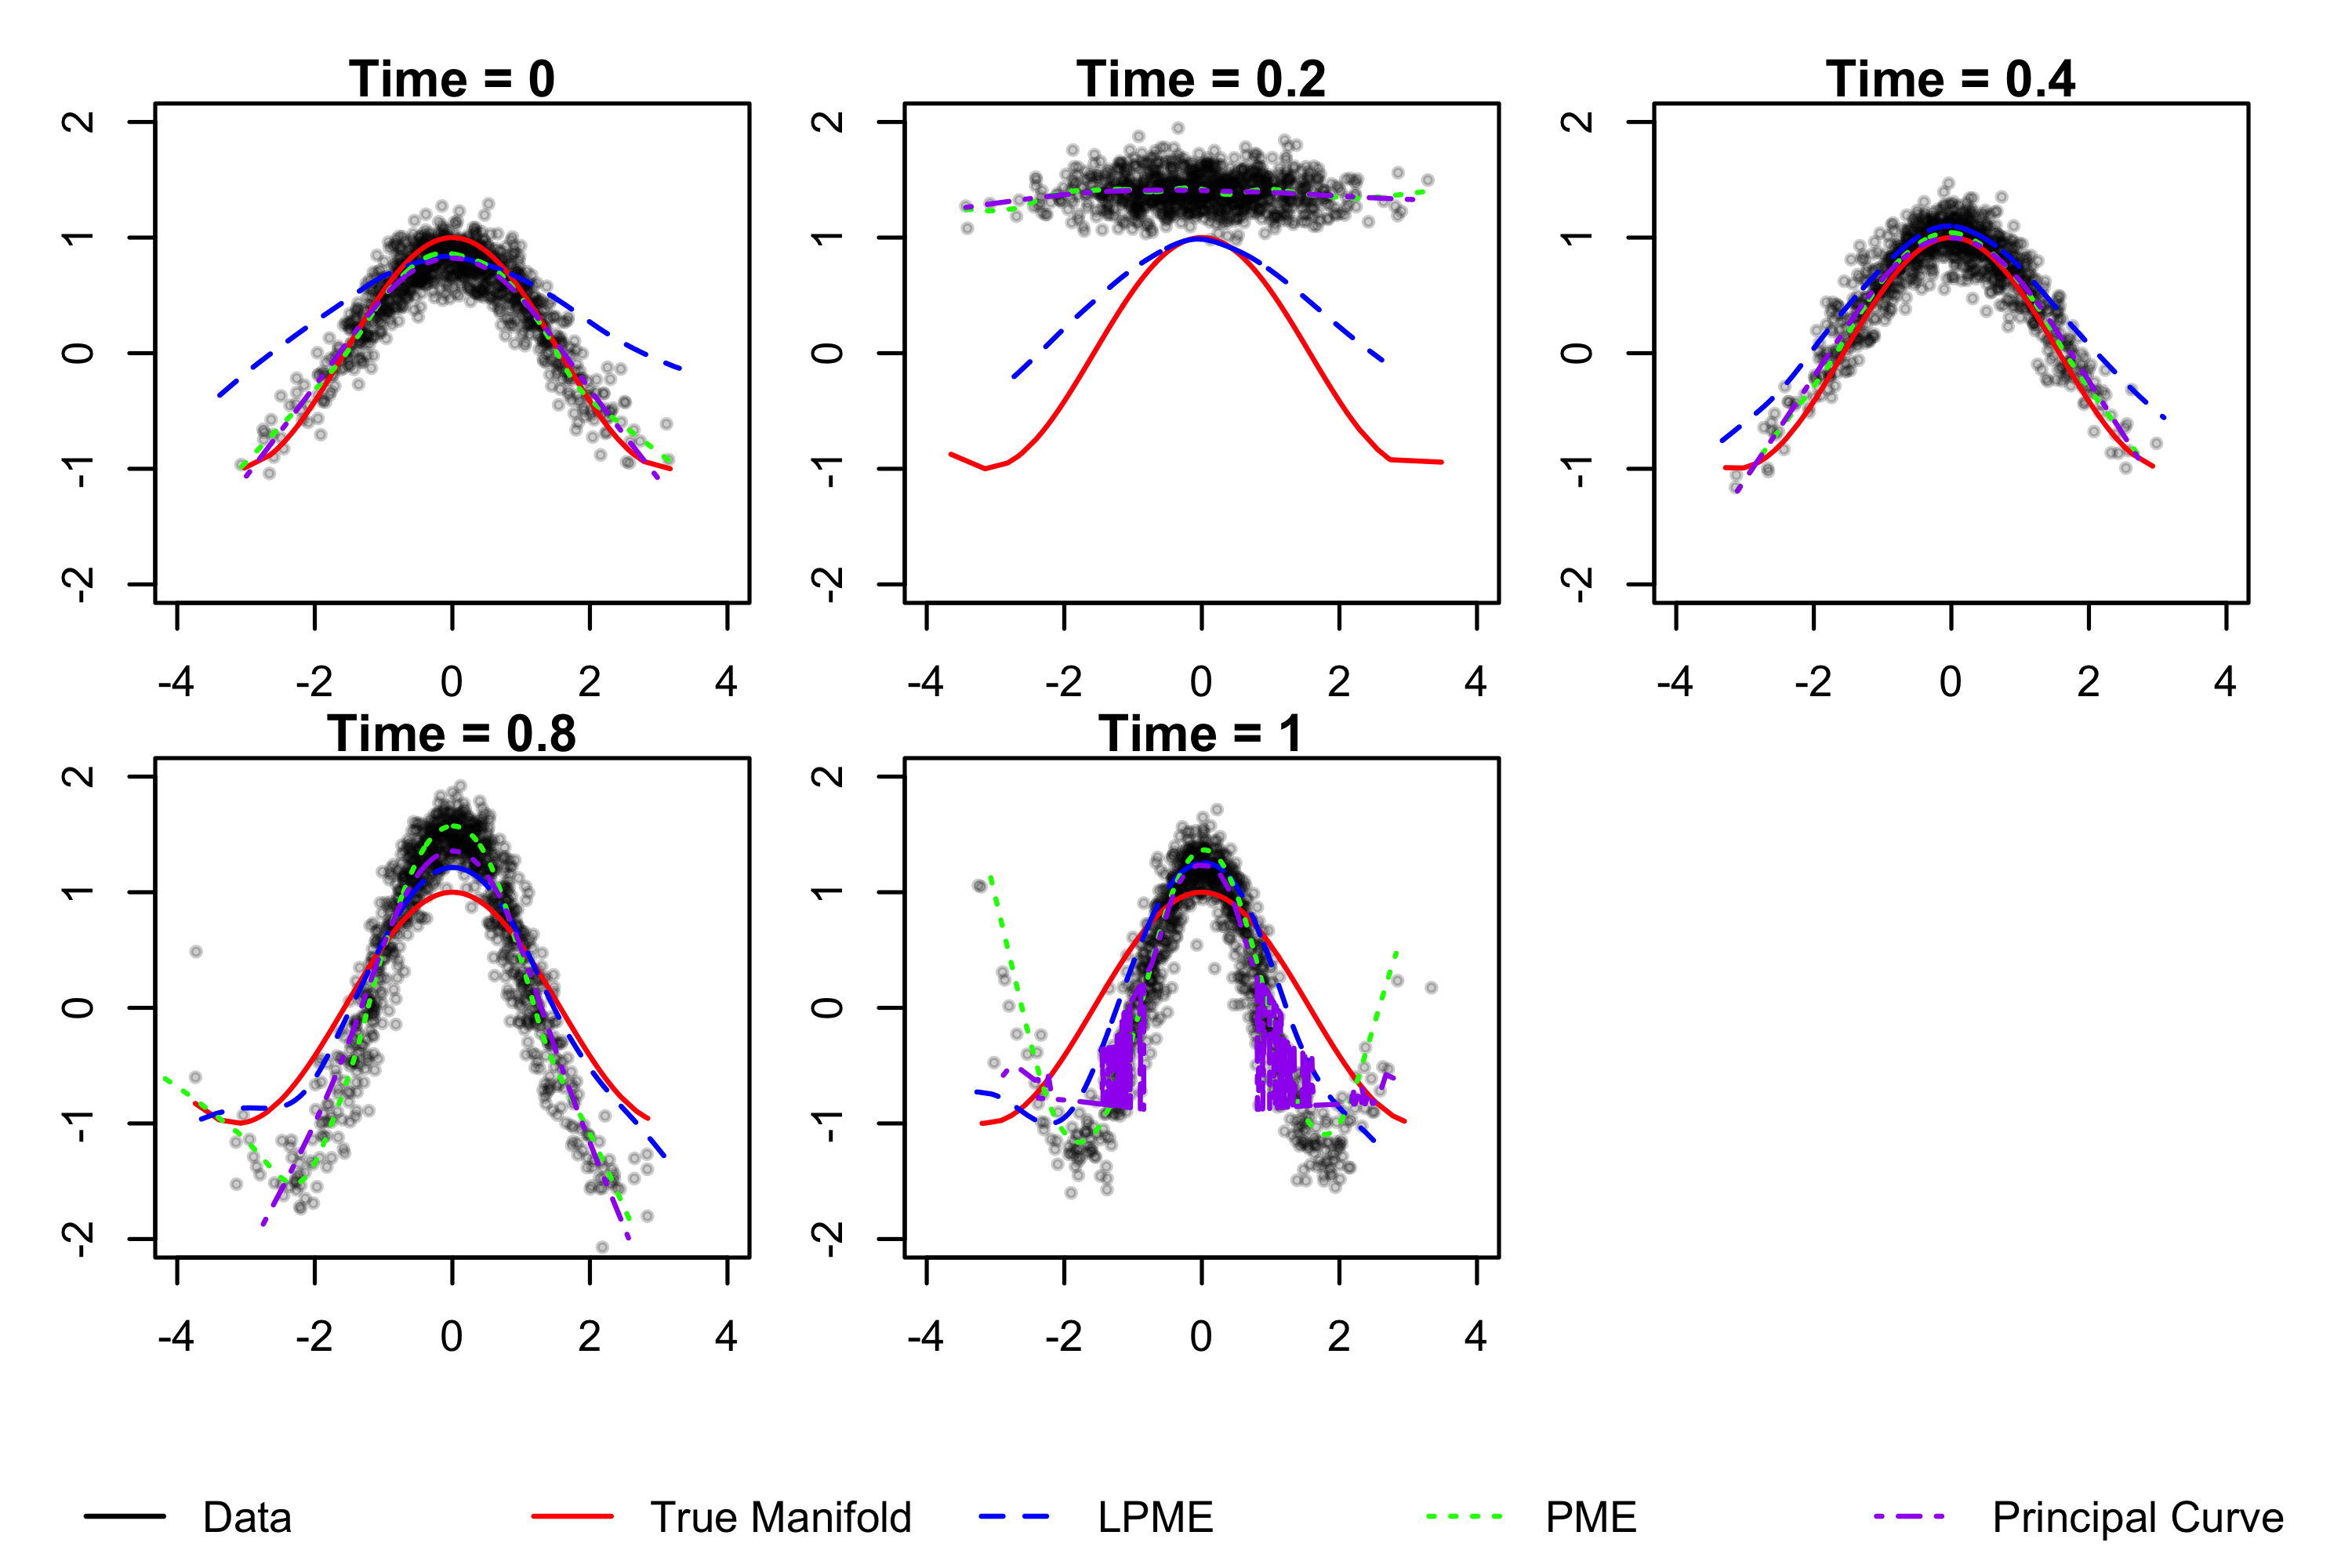
\includegraphics[width=\textwidth]{sim_case1}
  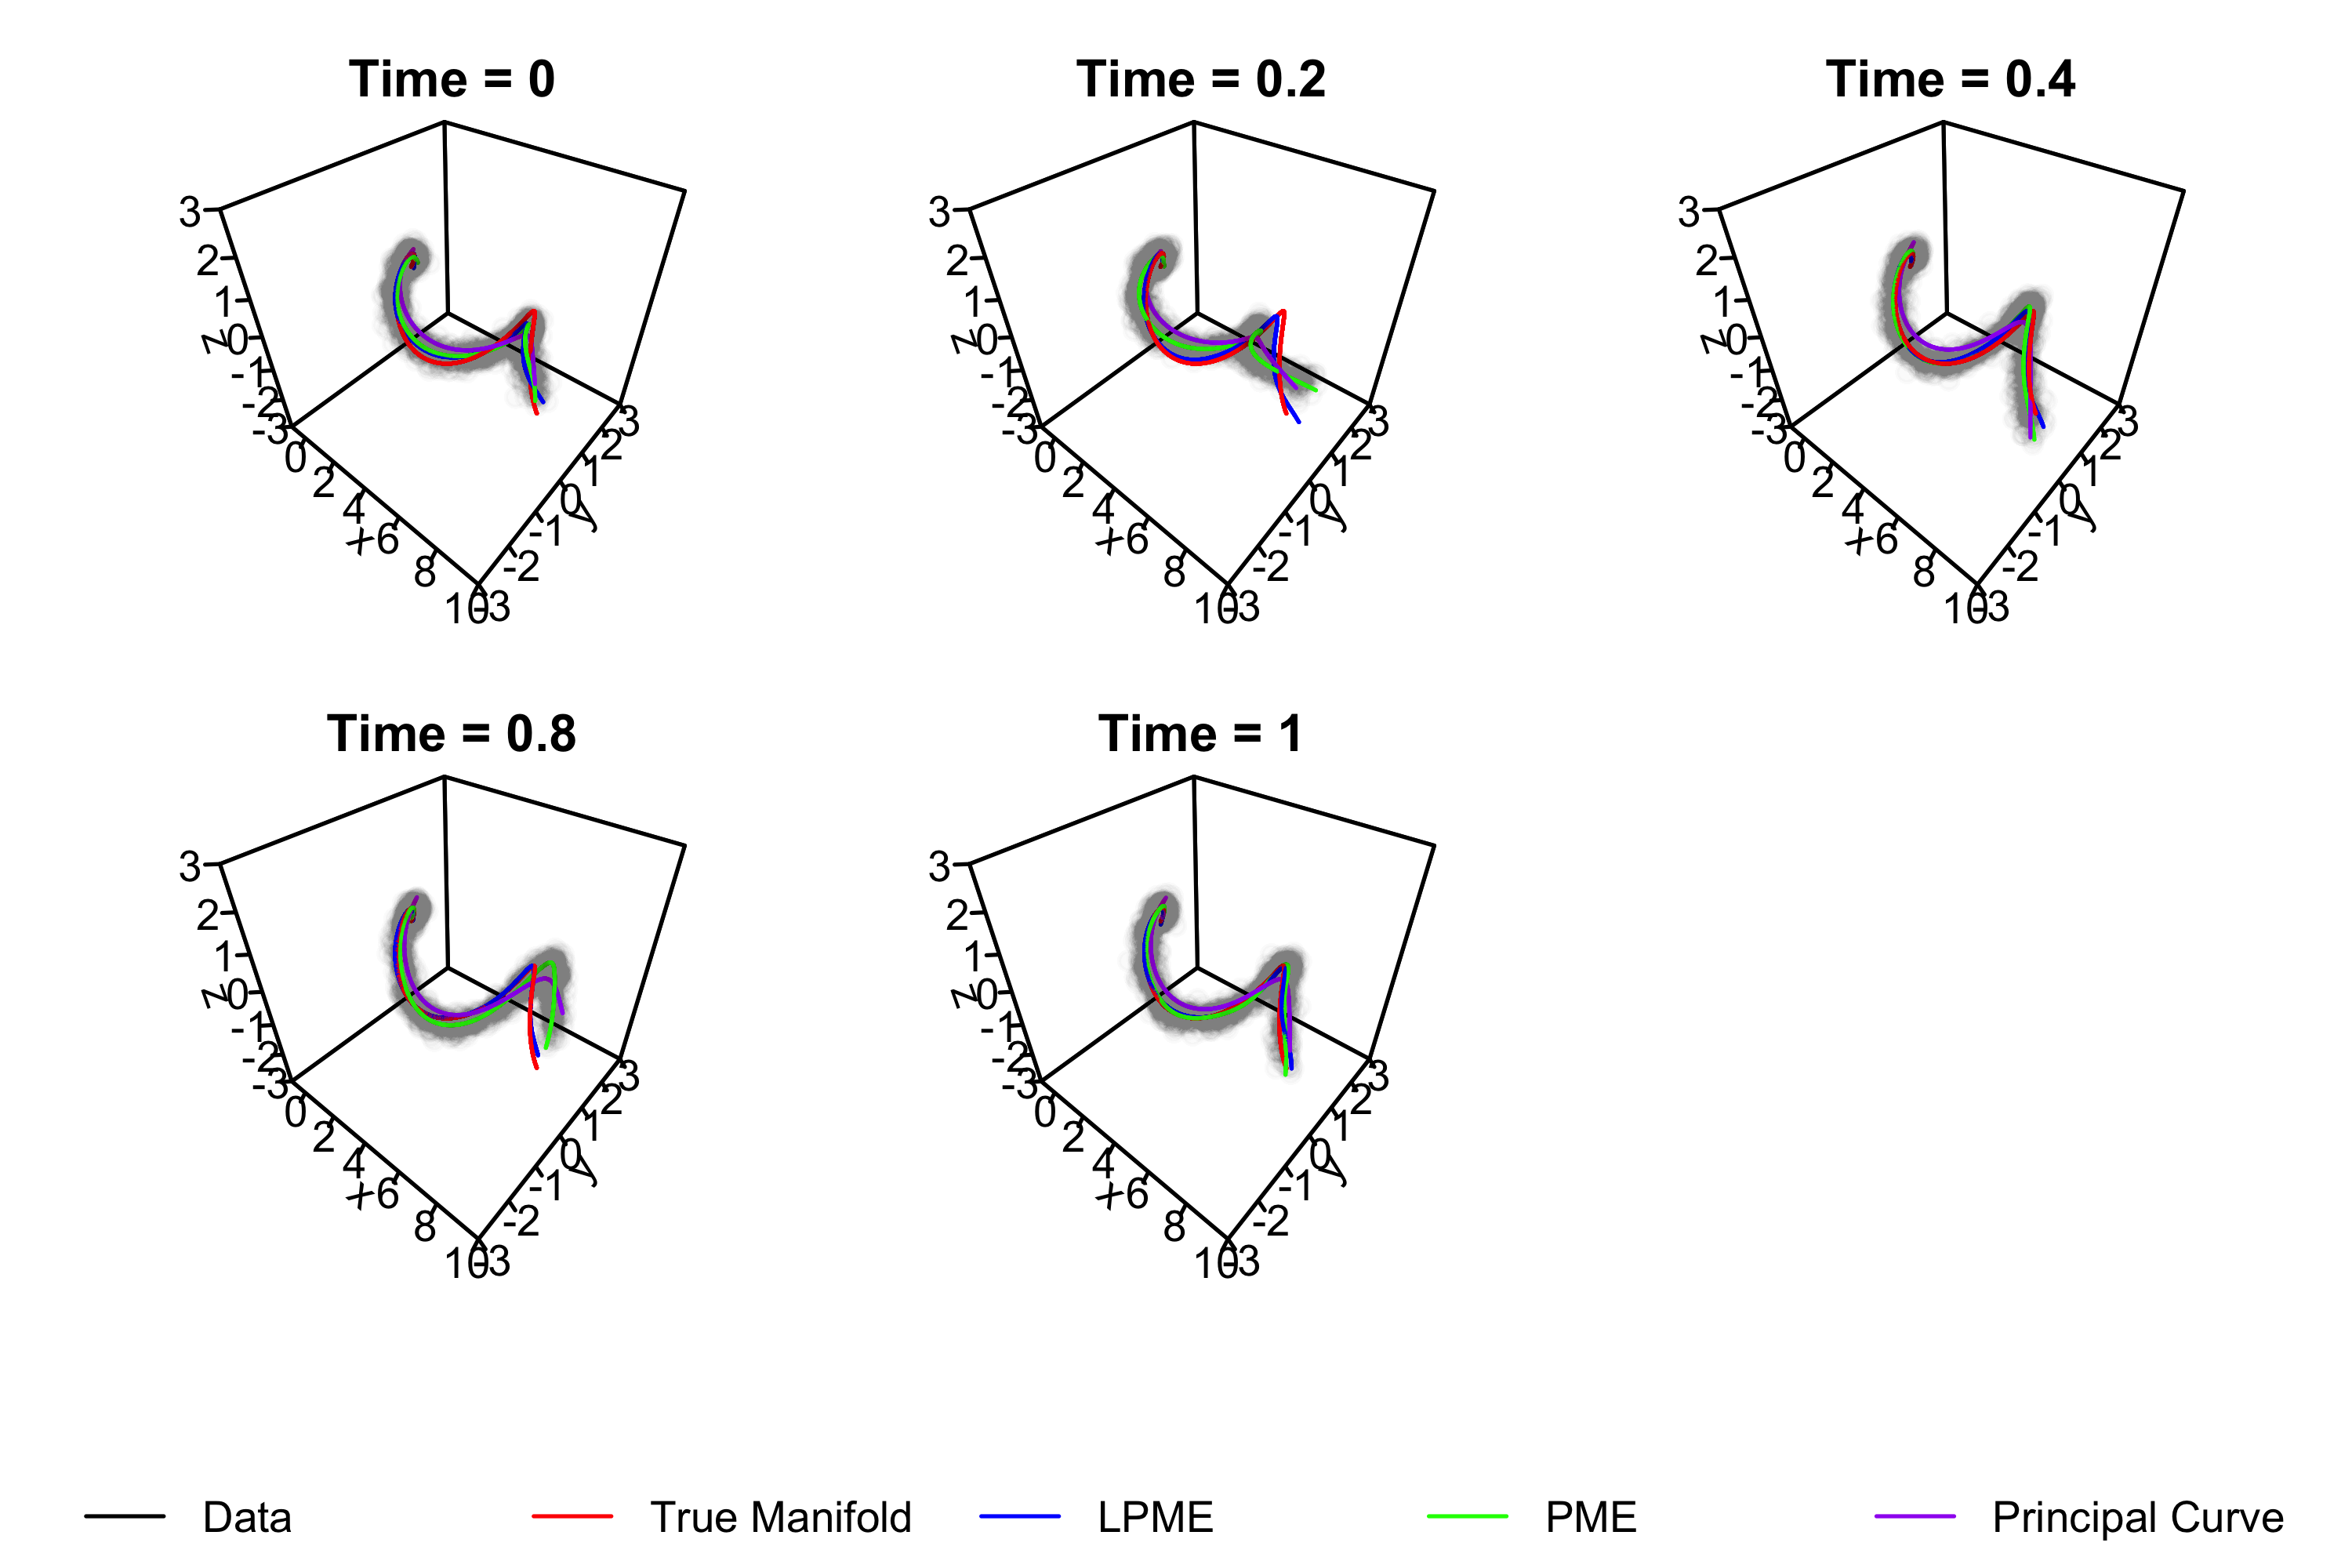
\includegraphics[width=\textwidth]{sim_case5}
  \caption{Simulation Cases 1 and 5.}
  \label{fig:sim_case1}
\end{figure}

\begin{figure}[h]
  \centering
  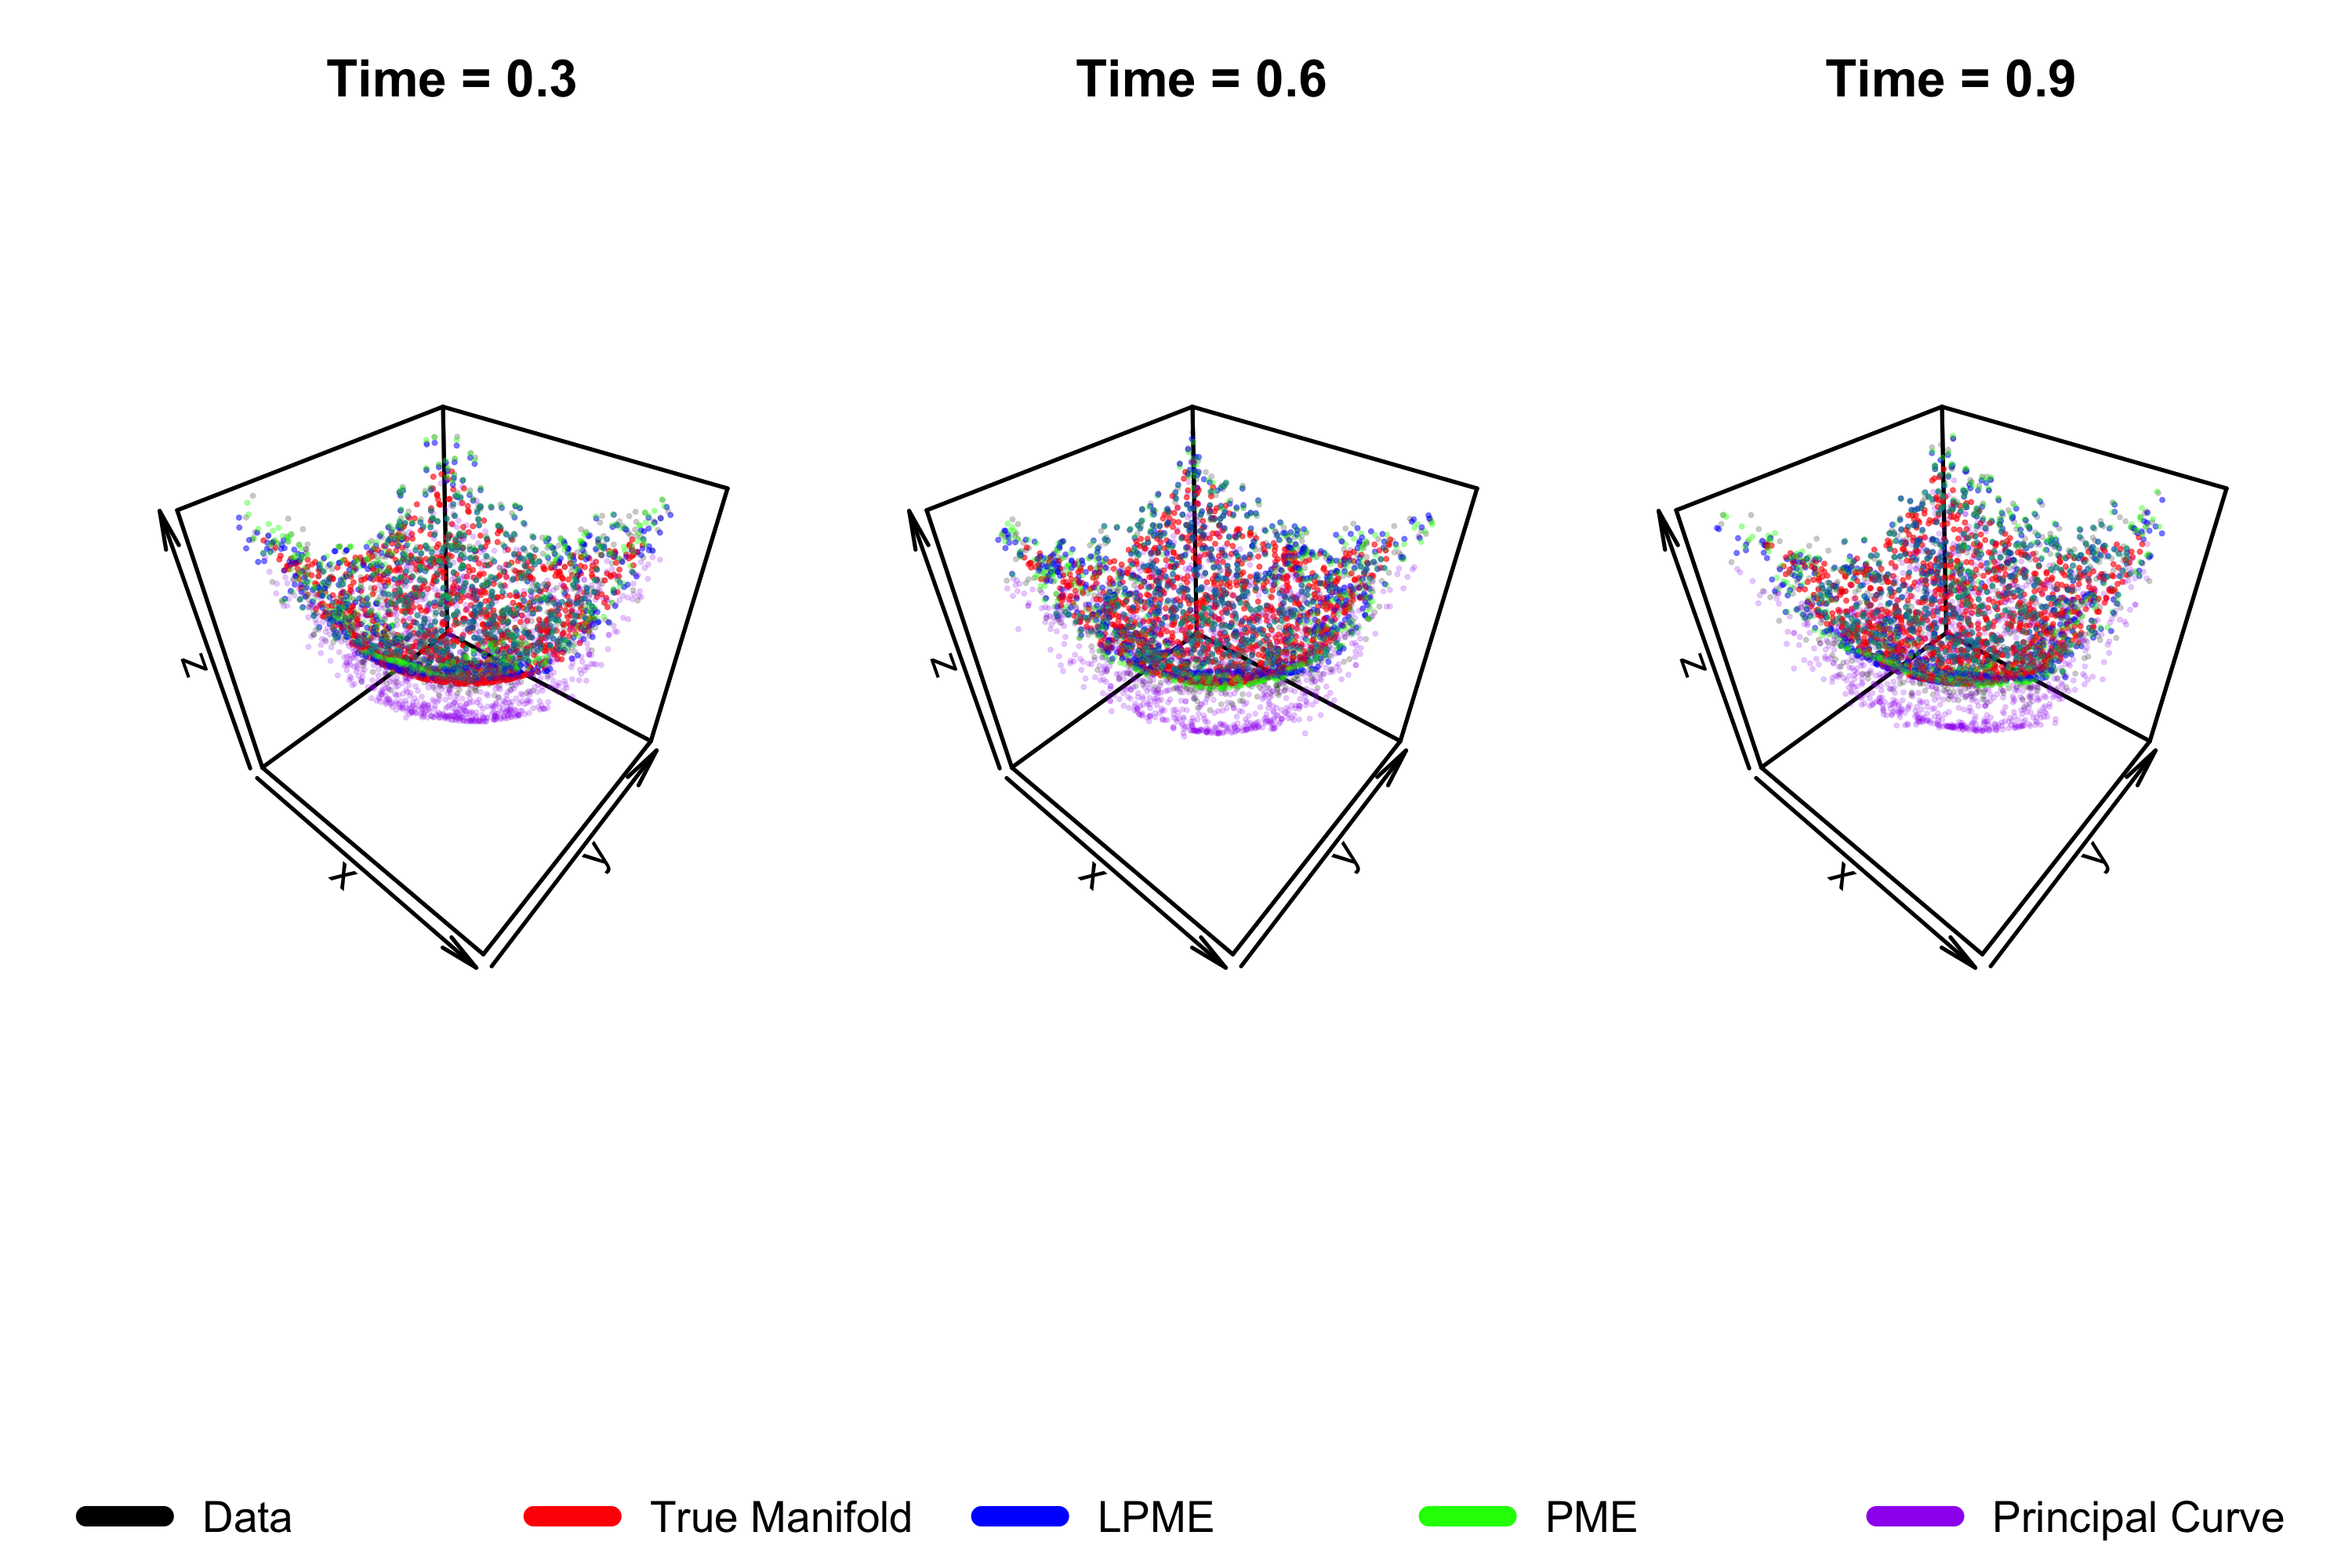
\includegraphics[width=\textwidth]{sim_case7}
  \caption{Simulation Case 6}
  \label{fig:sim_case6}
\end{figure}

The mean, median, standard deviation and interquartile range of the mean squared distance from the true underlying manifold values for the estimates of each approach, as well as for the data itself, are shown in Tables \ref{table:simulation_results_mean} and \ref{table:simulation_results_median}. Because the PME, principal curve, and principal surface methods each attempt to estimate the manifold in question at each individual time point without allowing other time points to inform these estimates, they should result in similar deviations from the true underlying manifold, with differences in error resulting primarily from differing performances in fitting to the observed data. Meanwhile, because the LPME approach accounts for all time points simultaneously, this approach should result in lower mean squared distance values.

The result summaries indicate that in most cases, LPME provides a substantial improvement in performance over the PME and principal curve approaches when estimating the underlying manifold. As seen clearly in Figure \ref{fig:sim_case1}, while the structure of the simulated data changes noticeably between time points, the LPME estimates, shown in blue, remain relatively stable over time. This contrasts to the estimates found by the PME and principal curve approaches, which are highly sensitive to the data observed at each given time point, as expected. This ultimately results in the LPME estimates remaining closer to the true underlying manifold, shown in red. Similar results hold in most of the other simulation cases.



\section{Longitudinal Segmentation of MRI images in Alzheimer's Disease Studies}\label{s:application}

As discussed previously, meaningful between-image error in estimates of subcortical structures is introduced during the process of segmenting MRI images. This section demonstrates how the LPME algorithm may be used to mitigate the effects of such noise on further analysis using these estimates. To achieve this, we used MRI data collected through the ADNI study, a longitudinal observational study with the goal of identifying imaging biomarkers to assess the progression of Alzheimer's disease (AD). 

While the original study included 200 cognitively healthy elderly individuals, 400 with mild cognitive impairment, and 200 with AD, for the purposes of demonstration we used $T_1$-weighted structural MRI images from eight study participants in the cognitively normal group (\cite{jack2008adni}). Follow-up duration for these participants ranged between approximately 16 months to 48 months, with imaging scheduled to be conducted at six month intervals. Individuals from the cognitively normal group were selected because drastic changes in the volume and shape of subcortical structures over the course of the study follow-up duration would be unexpected. Under this assumption, we attribute volumetric changes in a given structure to error introduced by the study procedure or the image segmentation process. Due to the changes experienced by those with Alzheimer's disease, we focused on the hippocampi of the selected individuals. 

Images were processed using FSL and ANTs via the \texttt{fslr} and \texttt{ANTsR} packages in \texttt{R}. Specifically, ANTs was used for bias correcting the images, and the FIRST method in FSL was used for image segmentation. Following image segmentation, the surfaces of each hippocampus were identified by finding the extreme voxels in each dimension with nonzero intensity readings. The estimated hippocampus surface positions were then standardized to a maximum distance of one from the origin in each dimension of Euclidean space and centered around the origin. Finally, the data were augmented with spherical coordinates in a manner similar to that described in Section \ref{s:LPME} to avoid the need to fit to a self-intersecting manifold.

%\zielinski{Reaching volume estimates from the LPME output is proving to be difficult.}

Results of fitting the PME and LPME algorithms on the surface of the left hippocampus of a single participant are shown in Figure \ref{fig:adni_result}. Visual inspection indicates that while there are slight differences between the shape shown in the data and the shape estimated by the LPME algorithm, the surface estimated by LPME appears to fit reasonably to the data. There are two main sources of discrepancies between the data and the LPME estimate. First, at time points where the observed surface changes orientation, as is visible between the first two time points, for example, the LPME estimates maintain a consistent orientation, reflecting the goal of encouraging stability in the structural estimates between time points. The second difference between the LPME estimates and the observed data can be seen at the sharper corners of the hippocampus, where the LPME estimates do not fully capture the severity of the curves seen in the observed data.

Figure \ref{fig:lhipp_cross_section} depicts cross sections of the observed hippocampus surface and the estimated surface obtained using LPME and PME at each individual time point. These cross sections illustrate the differences between the estimates reached by the PME and LPME algorithms, with the LPME-based estimate being generally less responsive to changes in the shape and orientation of the hippocampus between time points. This figure reiterates that both the PME and LPME algorithms are unable to capture the distinctive sharp curve in the structure at the upper-left corner of each of the plots. Additionally, we see that, along the upper-right edge of the surface, there is a spot where the estimated manifold intersects with itself. This is present for both the PME and LPME estimates, but appears to be more prevalent when using LPME. Notably, it also appears that the boundaries of the LPME-estimated surface tend to fall inside the boundaries of the PME-estimated surface, particularly at locations with the highest levels of curvature.

The hippocampus is a region with a relatively irregular shape, which may account for the differences in performance between the LPME algorithm when applied to simulated data and when applied to the hippocampus data. To understand how the approach performs when used with a more regularly shaped brain region, we also applied the PME and LPME algorithms to the surface of the left thalamus of the same healthy individuals described previously. Estimates of the surface of the thalamus were obtained from the MRI images using the same preprocessing and segmentation steps detailed above for the hippocampus data.

To understand the impacts of these discrepancies on the estimated volume of the regions, the volume of the hippocampus was approximated from the raw data and the estimates obtained by the PME and LPME algorithms at each time point. The volume estimation approach used here relies on counting the voxels contained within the boundary defined by the PME- or LPME-estimated embedding map, with each voxel having a known volume. The interior identification approach developed by \cite{mengPrincipalManifoldEstimation2021} is used to determine whether each voxel may be considered inside the surface of the structure or not. The code used to implement this approach is available at \texttt{https://github.com/rjzielinski/lpme-project}. The volume estimates can be found in Figure \ref{fig:lhipp_volumes}. Here, we see that volume estimates differ substantially depending on whether PME, LPME, or the raw data were used, with the LPME estimate resulting in the lowest volume computations.

The hippocampus is a region with a relatively irregular shape, which may account for the differences in performance between the LPME algorithm when applied to simulated data and when applied to the hippocampus data. To understand how the approach performs when used with a more regularly shaped brain region, we also applied the PME and LPME algorithms to the surface of the left thalamus of the same healthy individuals described previously. Estimates of the surface of the thalamus were obtained from the MRI images using the same preprocessing and segmentation steps detailed above for the hippocampus data.

Considering the same individual shown in Figures \ref{fig:adni_result} and \ref{fig:adni_cross_section}, results of fitting the PME and LPME algorithms to the surface of the left thalamus are shown in Figures \ref{fig:adni_lthal_result} and \ref{fig:adni_lthal_cross_section}. While the segmentation estimates of the thalamus do not show the same sort of deviations that are clearly visible for the hippocampus, the cross section plots shown in Figure \ref{fig:adni_lthal_cross_section} indicate that both the PME and LPME algorithms show a closer fit to the more regularly shaped thalamus surface than was achieved for the hippocampus. This is reflected in the smaller discrepancies between volume estimates, as seen in Figure \ref{fig:lthal_volumes}, though visible variations between time points remain.

\begin{figure}%
  \centering
  \subfloat[\centering Data]{{\includegraphics[height=22cm]{adni_plots/adni_data_plot}}}%
  \hfill
  \subfloat[\centering LPME Estimate]{{\includegraphics[height=22cm]{adni_plots/adni_lpme_plot}}}
  \hfill
  \subfloat[\centering PME Estimate]{{\includegraphics[height=22cm]{adni_plots/adni_pme_plot}}}

  \caption{Left Hippocampus, Cognitive Healthy ADNI Participant. The raw surface data, displayed in red, show slight changes in orientation that are absent in the LPME estimates, shown in blue. The estimates obtained by the PME and LPME algorithms appear unable to accurately capture the true shape of the structure at points with high levels of curvature.}
  \label{fig:adni_result}
\end{figure}



%\zielinski{Figure \ref{fig:adni_result} will continue to be improved, with the current version mainly serving as a placeholder.}

\begin{figure}[h]
  \centering
  \subfloat[\centering Left Hippocampus Cross Section]{\label{fig:lhipp_cross_sections} 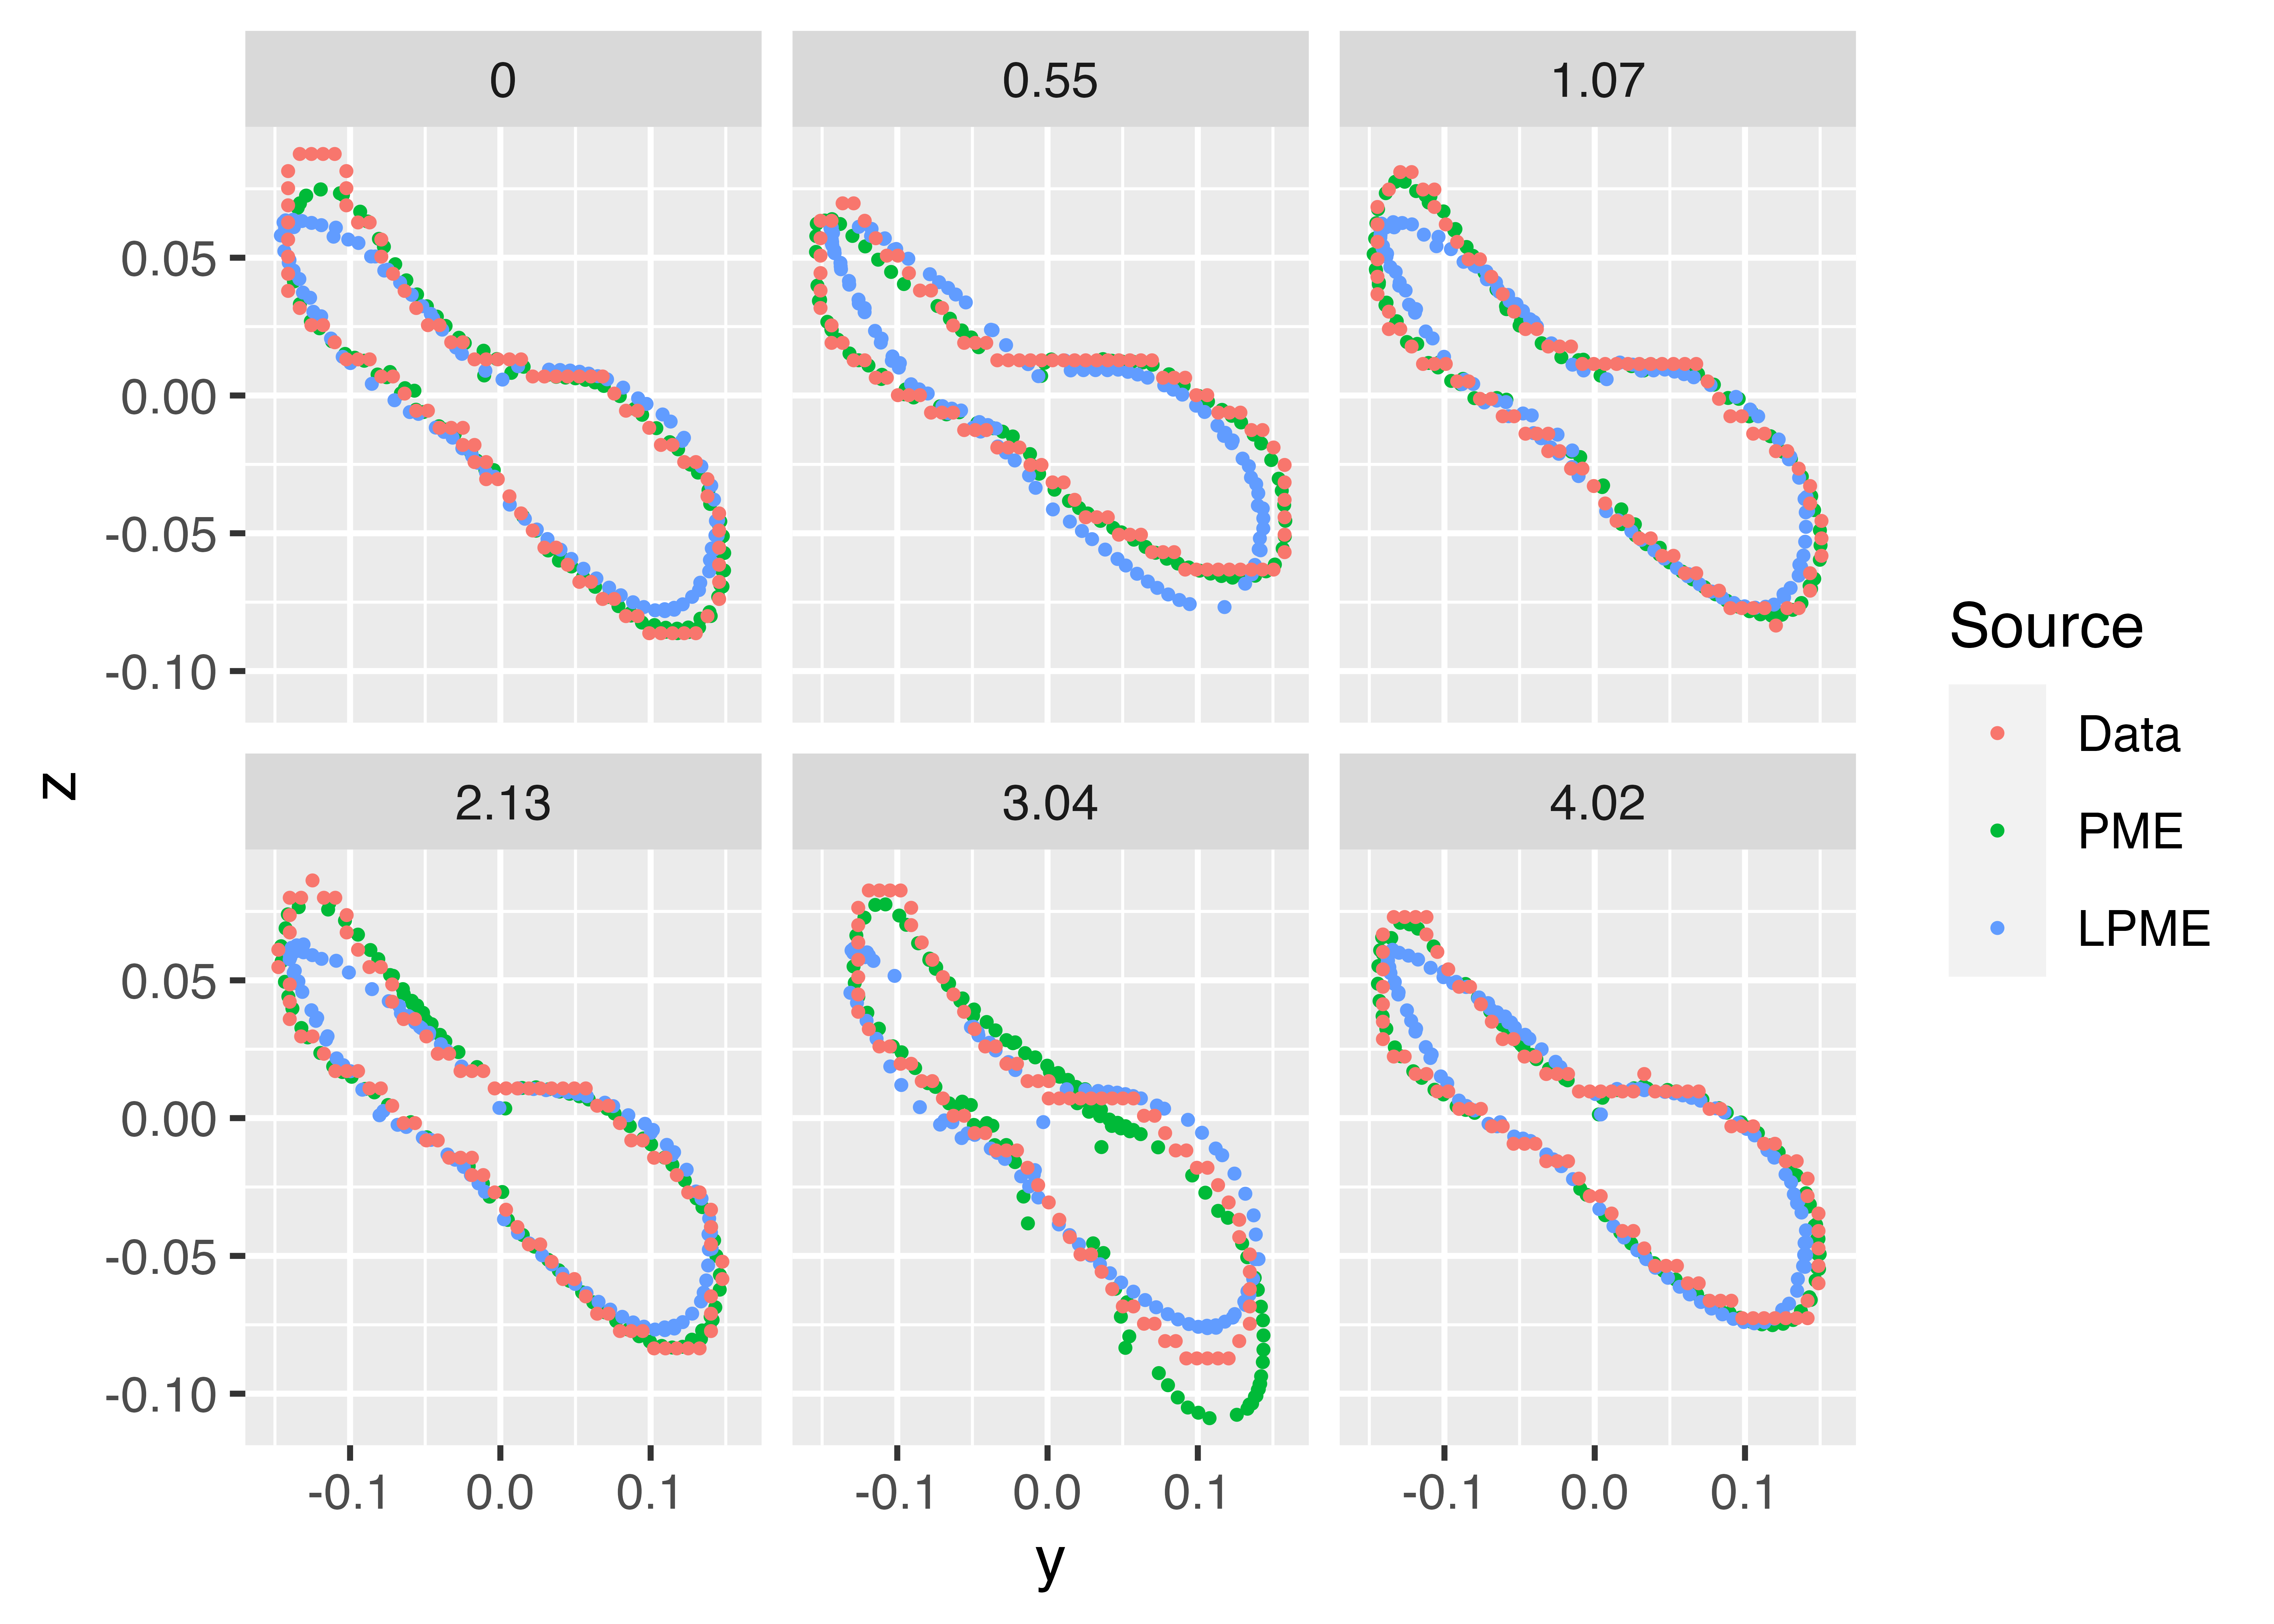
\includegraphics[width=8.5cm]{adni_plots/adni_cross_section}}%
  \hfill
  \subfloat[\centering Estimated Volumes]{\label{fig:lhipp_volumes} 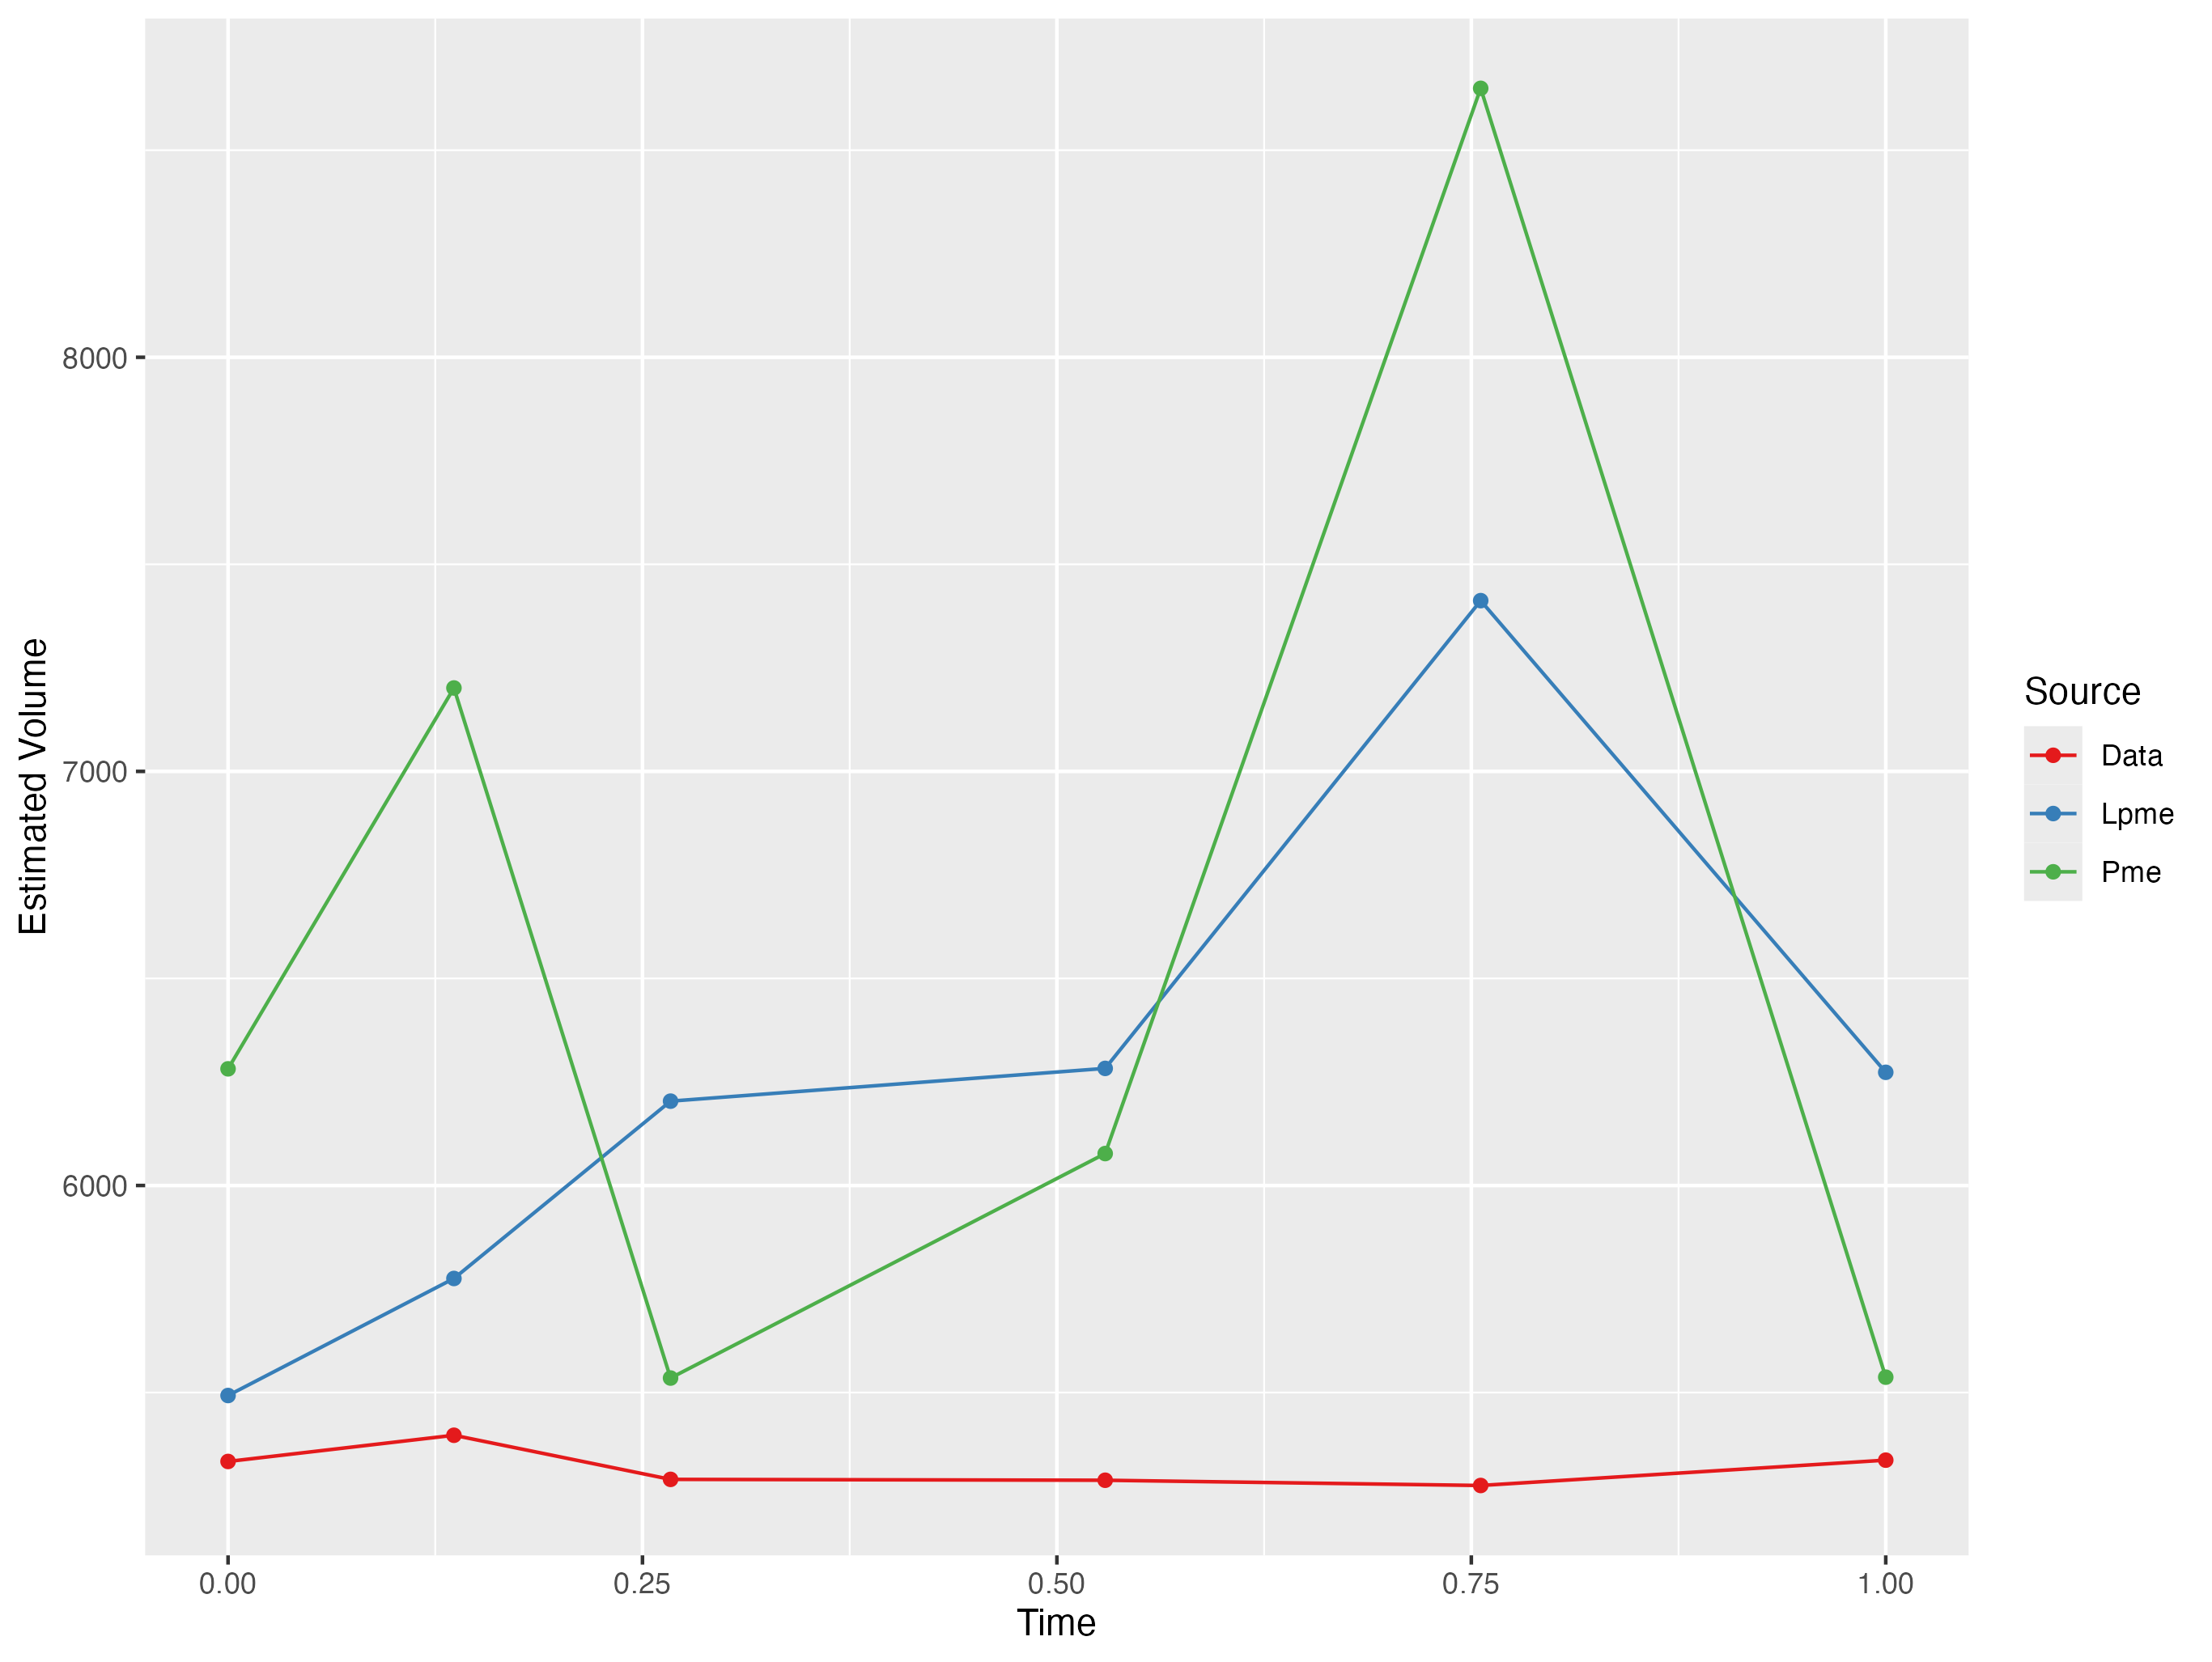
\includegraphics[width=8.5cm]{adni_plots/lhipp_volume}}
  \caption{Left Hippocampus Cross Section and Volume Estimates. In (a), we can see that the LPME-approximated embedding function, shown in blue, routinely falls inside the boundaries of surface in the observed data. In the fifth observation with $t=3.04$, the LPME-estimated surface has a gap in it, corresponding to an unexpectedly high volume estimate seen in (b). Volume estimates derived from the observed data are consistently higher than those obtained from the embedding functions of PME and LPME estimates, respectively.}
  \label{fig:adni_cross_section}
\end{figure}

\begin{figure}%
  \centering
  \subfloat[\centering Data]{{\includegraphics[height=22cm]{adni_plots/adni_lthal_data_plot}}}%
  \hfill
  \subfloat[\centering LPME Estimate]{{\includegraphics[height=22cm]{adni_plots/adni_lthal_lpme_isomap_plot}}}
  \hfill
  \subfloat[\centering PME Estimate]{{\includegraphics[height=22cm]{adni_plots/adni_lthal_pme_plot}}}

  \caption{Left Thalamus, Cognitive Healthy ADNI Participant}
  \label{fig:adni_lthal_result}
\end{figure}

\begin{figure}[h]
  \centering
  \subfloat[\centering Left Thalamus Cross Section]{\label{fig:lthal_cross_sections} 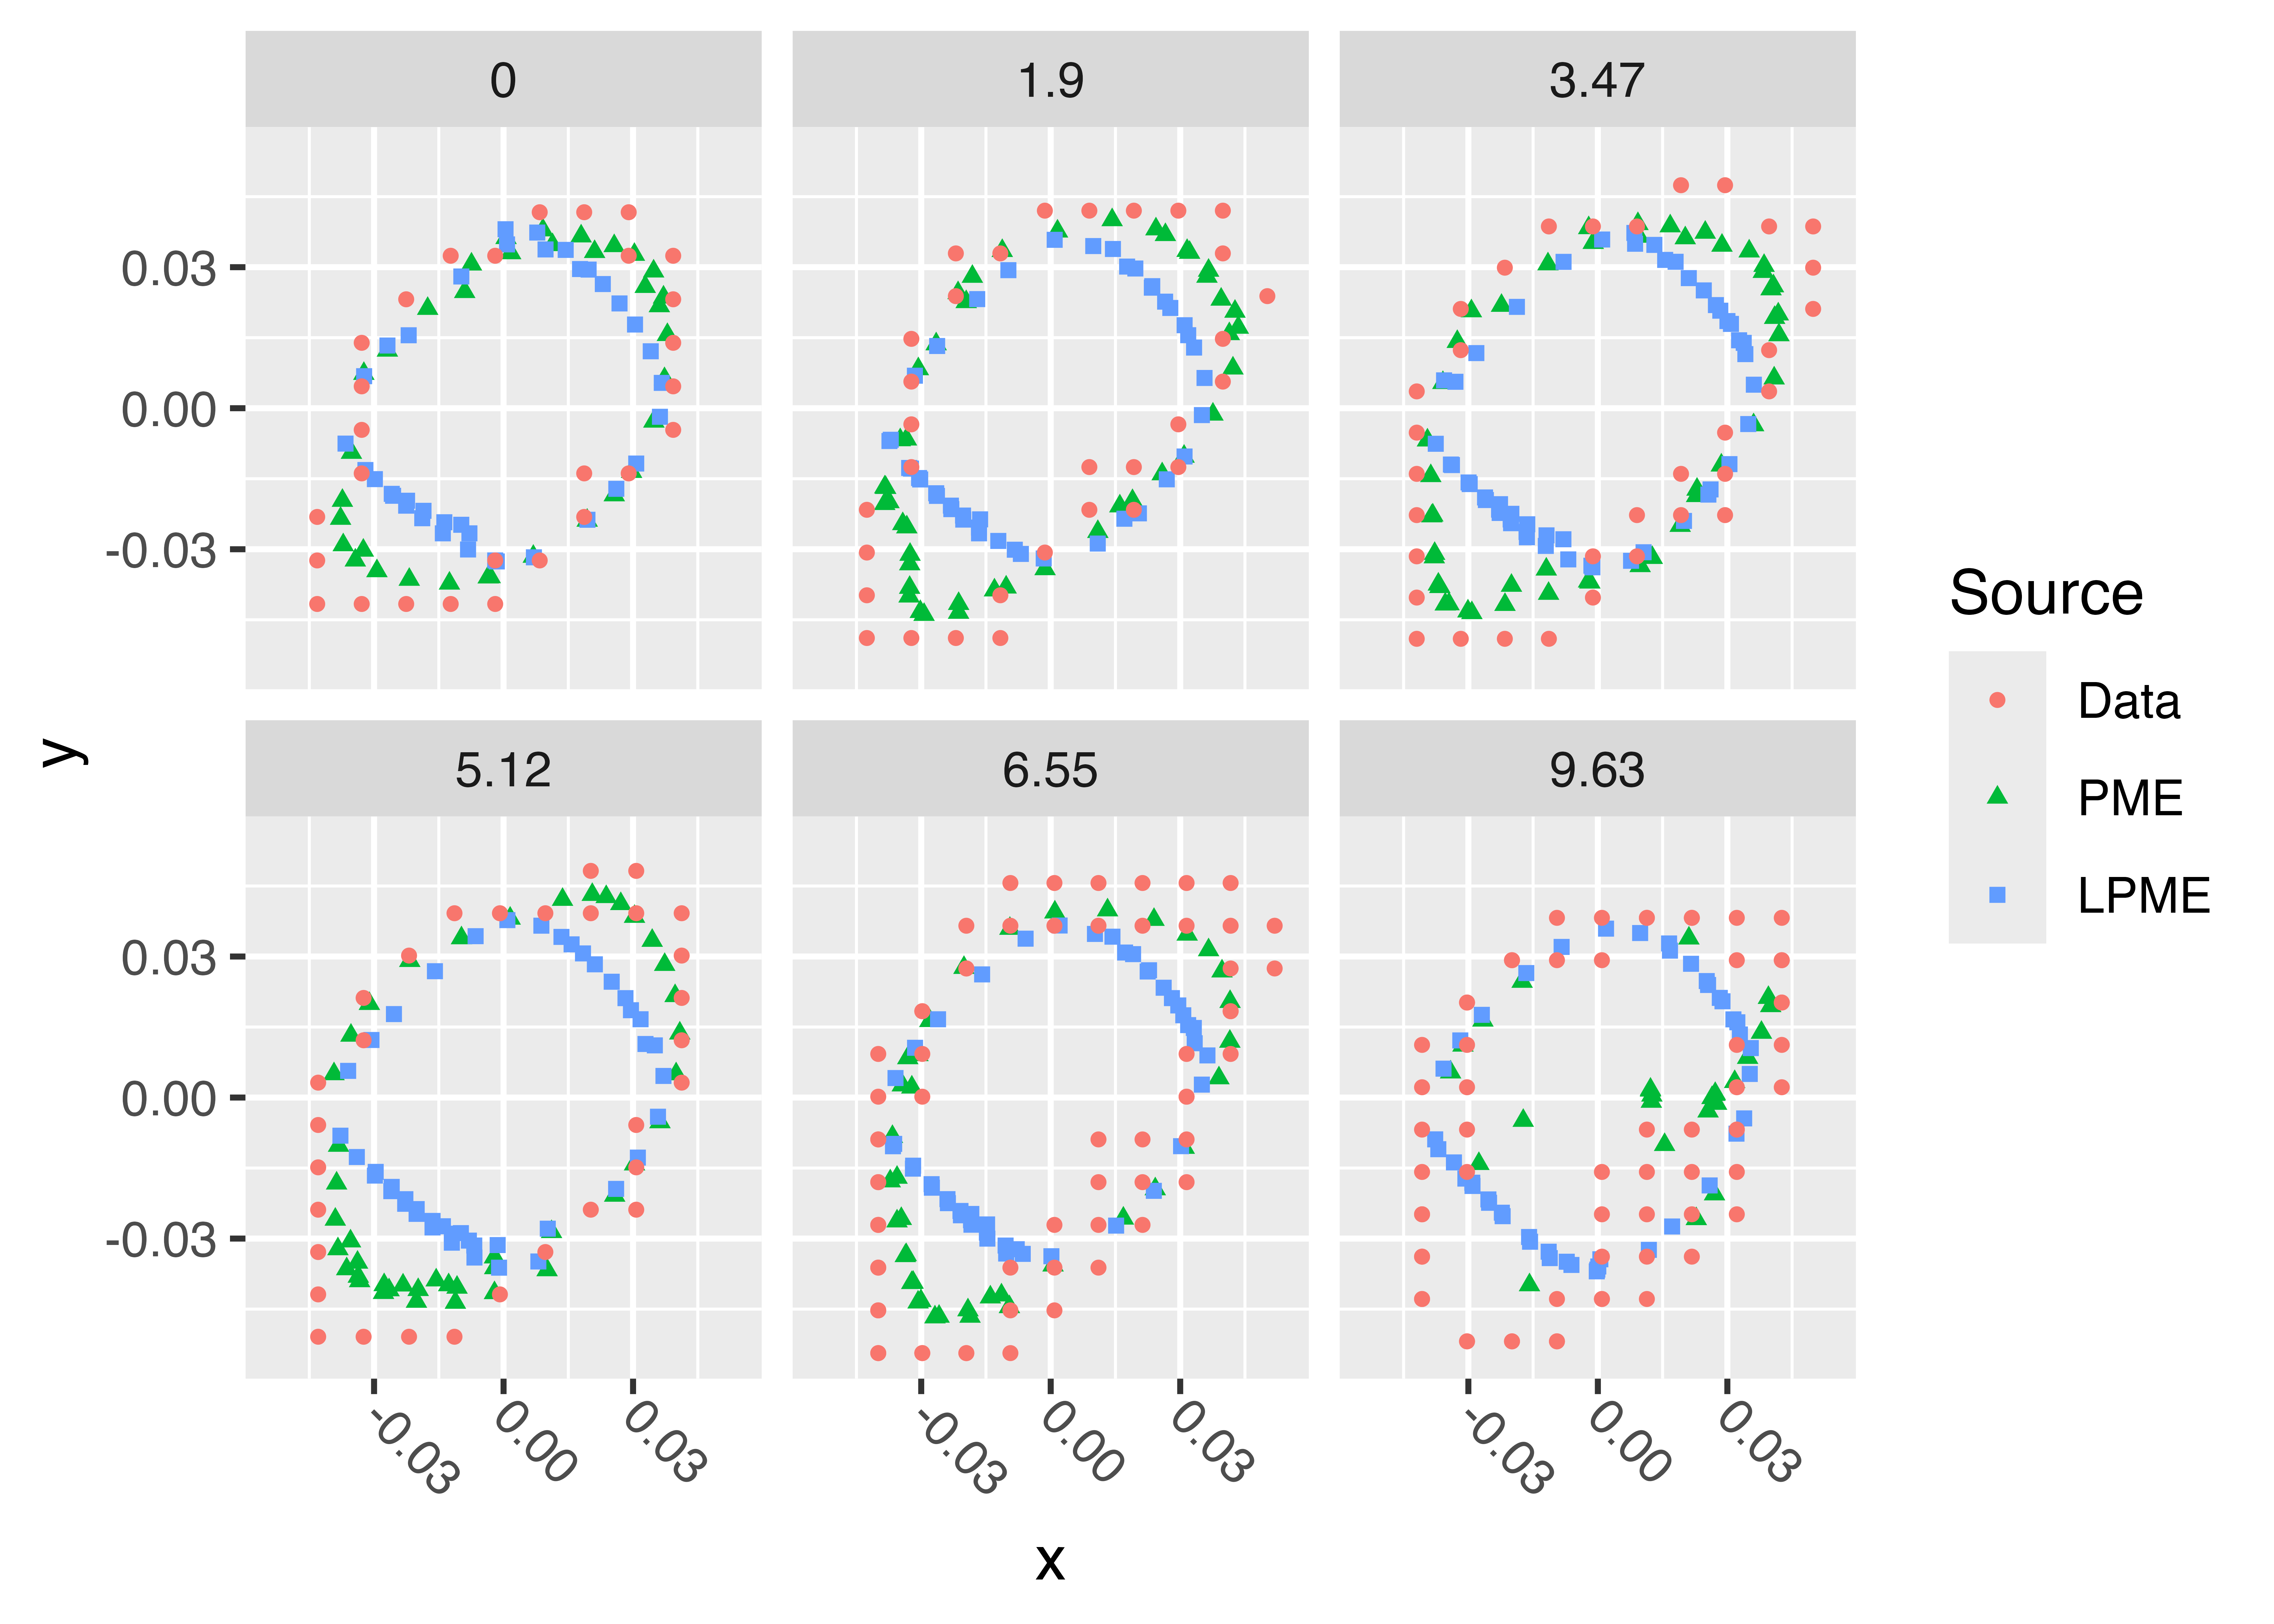
\includegraphics[width=8.5cm]{adni_plots/adni_lthal_cross_section}}%
  \hfill
  \subfloat[\centering Estimated Volumes]{\label{fig:lthal_volumes} 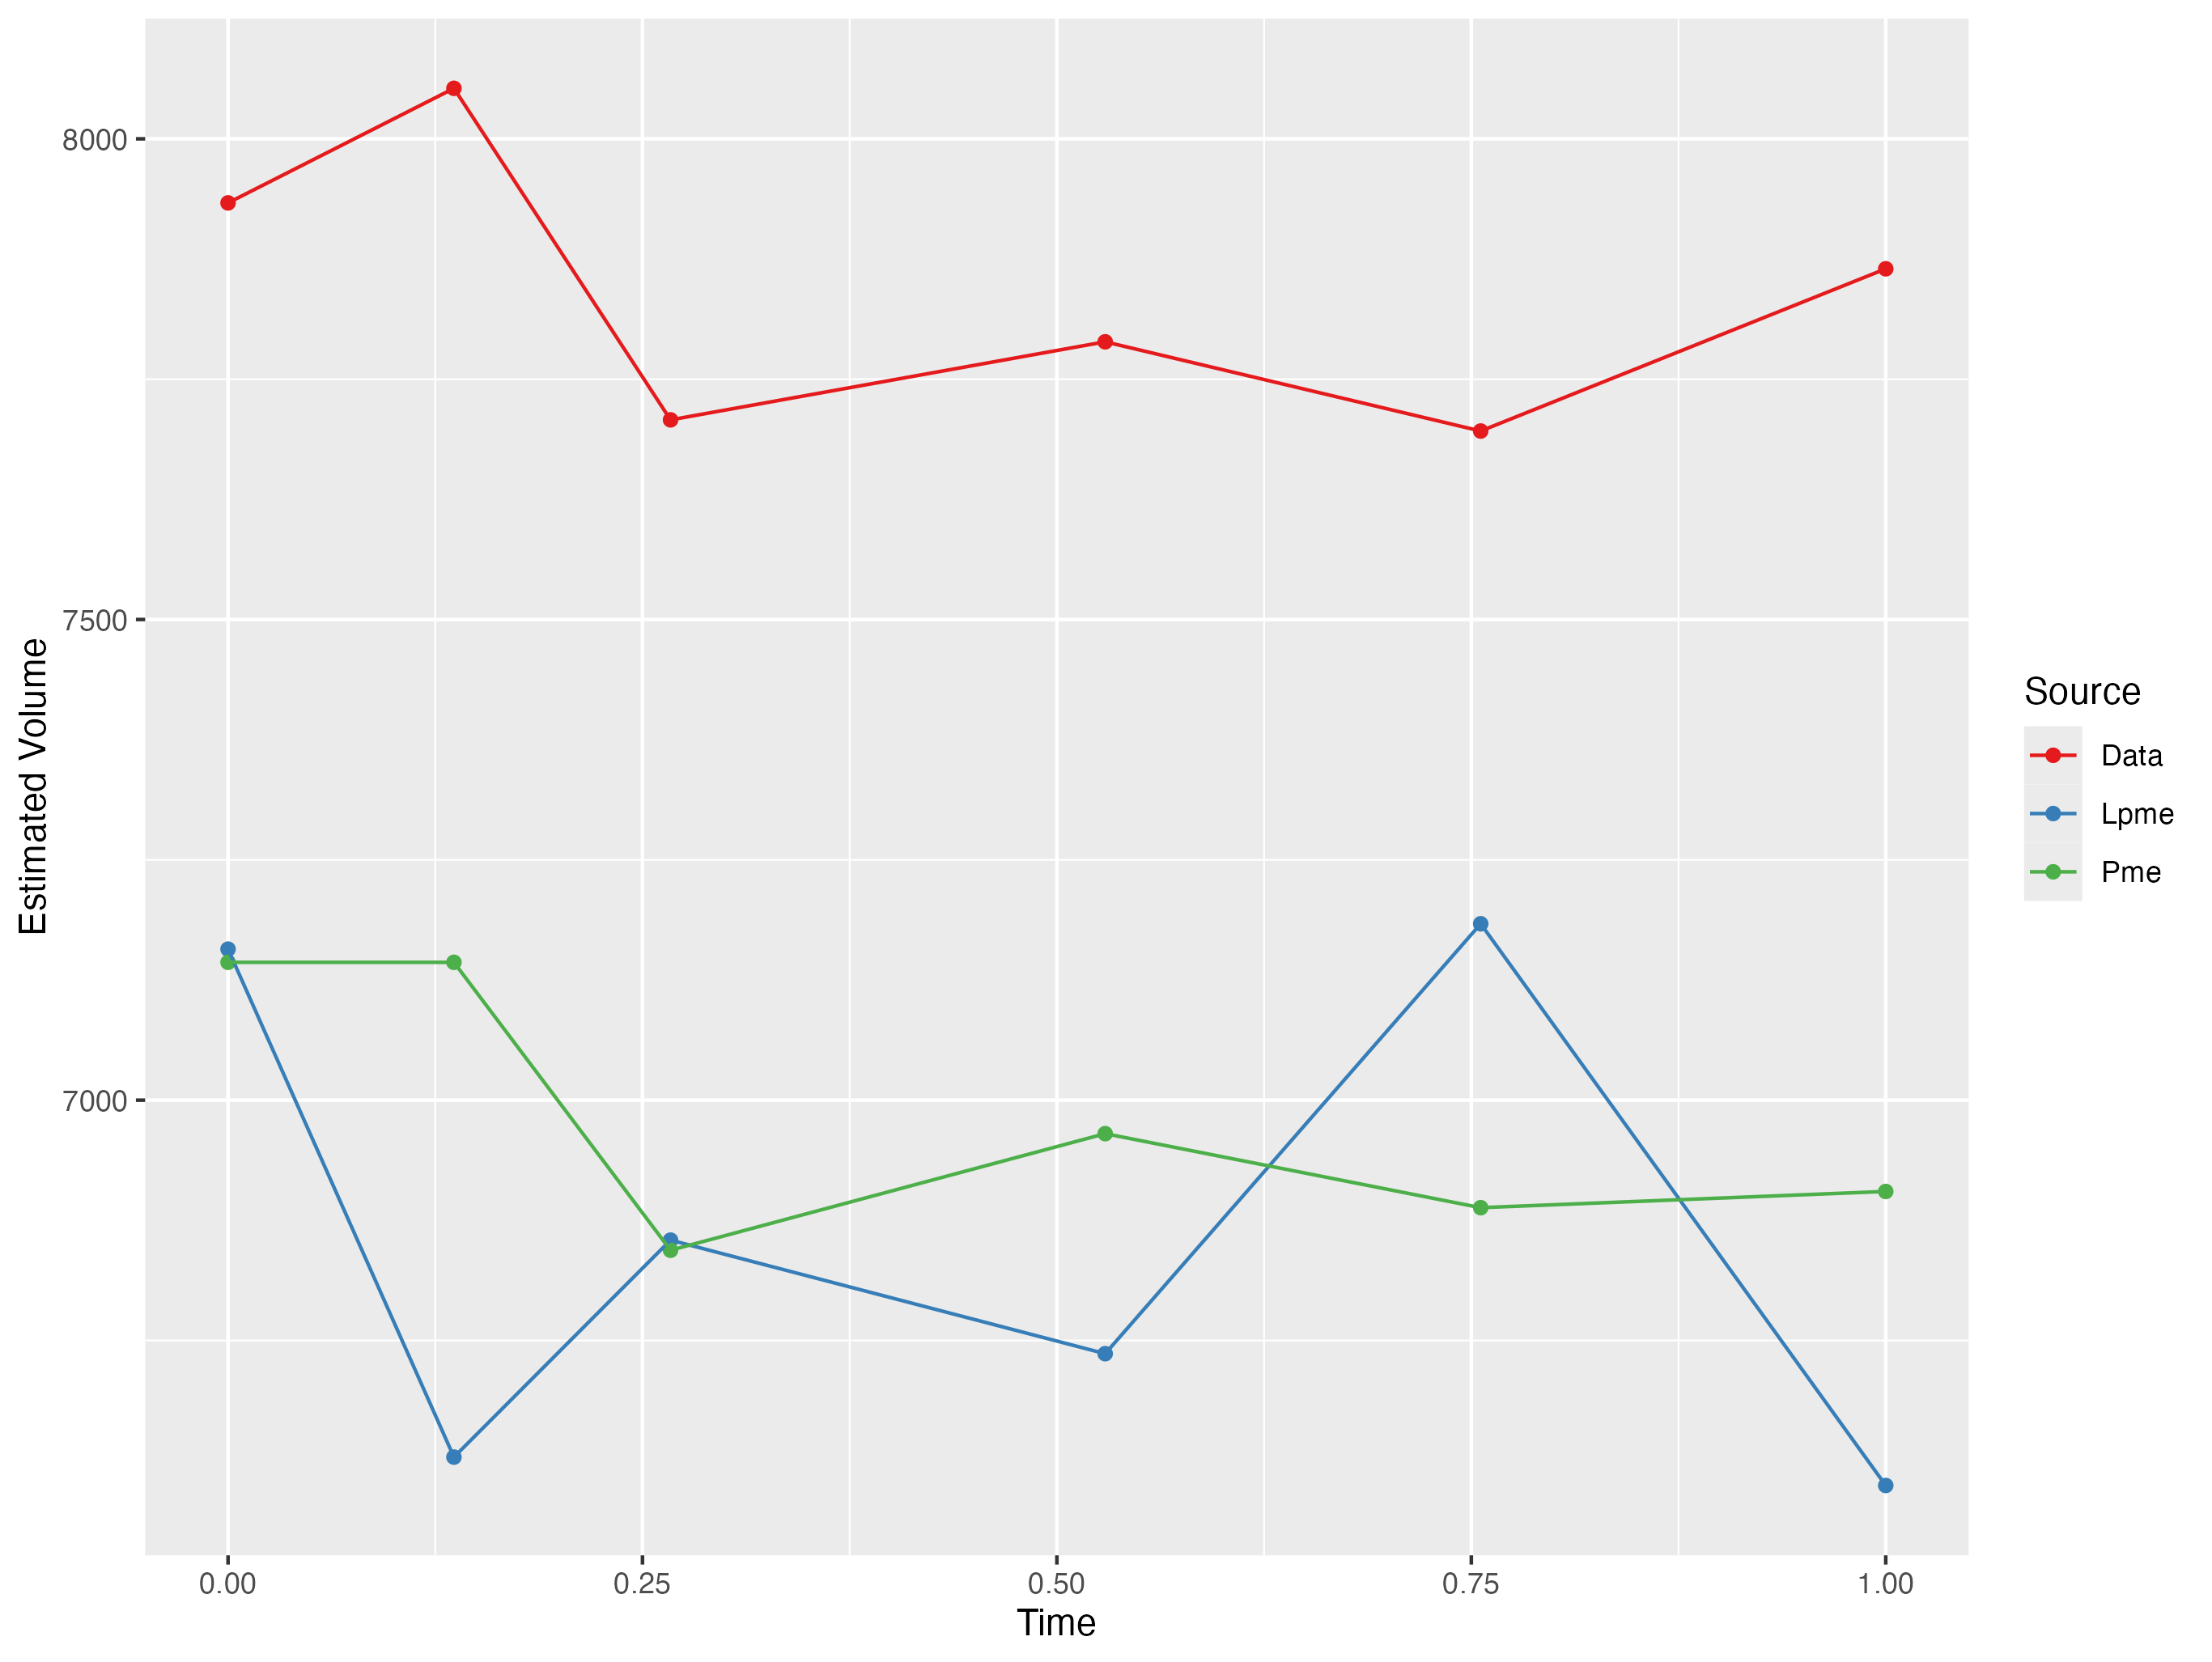
\includegraphics[width=8.5cm]{adni_plots/lthal_volume}}
  \caption{Left Thalamus Cross Section and Volume Estimates. In (a), the cross sectional plots indicate that the PME and LPME algorithms fit much more closely to the regularly shaped thalamus surface. The volume estimates in (b) show similar general trends to the hippocampus estimates, with the estimates reached using the observed data being higher than the PME- and LPME-based estimates. However, the differences between the estimates taken from the PME and LPME results are more comparable.}
  \label{fig:adni_lthal_cross_section}
\end{figure}


\section{Discussion}\label{s:discussion}

In this article, we propose an extension to the Principal Manifold Estimation algorithm introduced by \cite{mengPrincipalManifoldEstimation2021}, which may be used to model longitudinal changes in a low-dimensional manifold underlying high-dimensional data. To the best of our knowledge, this is the first time a nonlinear manifold learning method has been adapted to a general-purpose longitudinal setting. We also suggest a data augmentation approach that circumvents the inability to fit principal curve-based methods to self-intersecting manifolds in select settings. In simulated datasets where spurious changes in the structure to be estimated were introduced between time points, the LPME algorithm showed improved performance in recovering the underlying manifold when compared to a naive approach of applying either the PME or principal curve algorithms at each time point. This improvement was seen across several manifold types. 

It is key to note here that the MSD values shown in these tables compare the various models' projections onto the estimated manifold to the true values underlying the data the models are fit on. This means that a model that performs well using this metric may not perform well when comparing the model's projections onto the manifold with the data. In fact, if there is a high level of inter-observation noise, then we should expect an estimated manifold that closely follows the true underlying manifold to show a relatively poor fit to the data at any given time point. This largely explains why PME does not usually show better performance than the PC/PS methods using this metric - both approaches are trying to estimate a curve or surface using the data available at a given time point, which may have noise introduced that increases the distance to the true manifold. When comparing the fit of the PME and PC methods to the simulated data, PME tends to show improvement in the median MSD, with elevated mean MSD levels compared to principal curves.

While the LPME algorithm demonstrated strong performance in a number of settings, it also has several limitations. First, because the method explicitly builds on the results of an estimate provided by the PME algorithm, the LPME algorithm will only fit properly in situations where PME fits properly. Because the output of PME is dependent on the success of its initial parameterization, in practice this limits the success of LPME to situations where Isomap performs well, which excludes nonconvex manifolds, manifolds that have holes, or manifolds that have too high a level of curvature. The option to use alternative methods, such as Locally Linear Embedding or Laplacian Eigenmaps, to generate the initial parameterization for the PME algorithm may help to alleviate this concern. Opportunities also exist to improve the tuning of the initialization method, which may result in better performance, especially when considering data with different levels of noise present.  

A second limitation is that the LPME method requires relative stability in the overall shape of the structure being fit over time. Thus, while this algorithm can be useful for separating meaningful changes in a manifold over time from inter-observation error, it will be unable to fit in situations where the error between observations is too substantial. How restrictive this requirement is depends largely on the area of application. When used to estimate subcortical surfaces as suggested here, this tends not to be overly restrictive, as changes in the shape and size of a subcortical structure, while clinically meaningful, tend to be relatively small in magnitude compared to their defining features.

Another limitation stems from the performance of the LPME method on the hippocampus surfaces obtained from the ADNI dataset. It is clear that neither the PME nor the LPME estimates were able to fully capture the distinctive curved structure of the hippocampus. This shortcoming could potentially be addressed in several ways. First, as discussed above, the manifold learning method used in the initialization step of the PME algorithm, or the parameters of that method could be adjusted to better meet the needs of the specific manifold being estimated. Second, while a simple grid search is used to select the optimal value of the smoothing parameter in both the PME and LPME algorithms, it is possible that an improved search method would yield results that are more sensitive to the nuances of the structure being estimated. Finally, it may be possible to manipulate the manifold to be easier to estimate through adjustments to the data augmentation process, as described in Section \ref{s:LPME}. The volume estimates obtained from the outputs of the PME and LPME algorithms reflected the insufficient fit of these algorithms to the hippocampus data. However, the volume estimation process includes ad hoc approaches to address missing data, and the high level of variability in the estimated volumes of the thalamus despite visual indications of improved fit to this data suggests that this approach may itself be contributing to this variability. Further testing of this approach will be needed before the LPME algorithm will be viable for approximating the volume of brain regions.

Additional work will also be necessary to more thoroughly explore the data augmentation approach proposed in this article and its capabilities. The simple calculations used here allowed the PME and LPME algorithms to estimate self-intersecting manifolds that would not previously have been estimable by these methods. However, while the use of polar and spherical coordinates addressed a problem posed by well-behaved circular structures, it would not necessarily apply easily to the hippocampus or more complex structures, such as a figure 8 shape, or even rounded structures with large variations in the radius, which would result in several points sharing an angle from the origin. The development of a procedure to handle these considerations would greatly expand the potential use cases for this approach, thus allowing principal manifold-based methods to be used in a wider range of situations. While the approach described in this article is limited to the estimation of manifolds from observations taken from a single structure over time, the further extension of this method to manifold estimation for groups of similar structures would also be of interest.

%\meng{FYI, we may also apply Gaussian process regression (GPR) to smooth the time direction. The smoothness can be represented by the covariance kernel we use in the GPR. For example, we may apply the Gaussian or \href{https://en.wikipedia.org/wiki/Matern_covariance_function}{Matérn} kernels. The taste of the GPR is similar to \cite{dunsonInferringManifoldsNoisy2022}, and we may cite \cite{dunsonInferringManifoldsNoisy2022}.}
\newpage

\nocite{*}
%\bibliographystyle{plain}
%\bibliography{references}
\printbibliography

\end{document}
